% Options for packages loaded elsewhere
\PassOptionsToPackage{unicode}{hyperref}
\PassOptionsToPackage{hyphens}{url}
%
\documentclass[
  11pt,
]{book}
\usepackage{lmodern}
\usepackage{amssymb,amsmath}
\usepackage{ifxetex,ifluatex}
\ifnum 0\ifxetex 1\fi\ifluatex 1\fi=0 % if pdftex
  \usepackage[T1]{fontenc}
  \usepackage[utf8]{inputenc}
  \usepackage{textcomp} % provide euro and other symbols
\else % if luatex or xetex
  \usepackage{unicode-math}
  \defaultfontfeatures{Scale=MatchLowercase}
  \defaultfontfeatures[\rmfamily]{Ligatures=TeX,Scale=1}
\fi
% Use upquote if available, for straight quotes in verbatim environments
\IfFileExists{upquote.sty}{\usepackage{upquote}}{}
\IfFileExists{microtype.sty}{% use microtype if available
  \usepackage[]{microtype}
  \UseMicrotypeSet[protrusion]{basicmath} % disable protrusion for tt fonts
}{}
\makeatletter
\@ifundefined{KOMAClassName}{% if non-KOMA class
  \IfFileExists{parskip.sty}{%
    \usepackage{parskip}
  }{% else
    \setlength{\parindent}{0pt}
    \setlength{\parskip}{6pt plus 2pt minus 1pt}}
}{% if KOMA class
  \KOMAoptions{parskip=half}}
\makeatother
\usepackage{xcolor}
\IfFileExists{xurl.sty}{\usepackage{xurl}}{} % add URL line breaks if available
\IfFileExists{bookmark.sty}{\usepackage{bookmark}}{\usepackage{hyperref}}
\hypersetup{
  hidelinks,
  pdfcreator={LaTeX via pandoc}}
\urlstyle{same} % disable monospaced font for URLs
\usepackage[margin=0.8in]{geometry}
\usepackage{graphicx,grffile}
\makeatletter
\def\maxwidth{\ifdim\Gin@nat@width>\linewidth\linewidth\else\Gin@nat@width\fi}
\def\maxheight{\ifdim\Gin@nat@height>\textheight\textheight\else\Gin@nat@height\fi}
\makeatother
% Scale images if necessary, so that they will not overflow the page
% margins by default, and it is still possible to overwrite the defaults
% using explicit options in \includegraphics[width, height, ...]{}
\setkeys{Gin}{width=\maxwidth,height=\maxheight,keepaspectratio}
% Set default figure placement to htbp
\makeatletter
\def\fps@figure{htbp}
\makeatother
\setlength{\emergencystretch}{3em} % prevent overfull lines
\providecommand{\tightlist}{%
  \setlength{\itemsep}{0pt}\setlength{\parskip}{0pt}}
\setcounter{secnumdepth}{5}
\setlength{\parskip}{1em} \linespread {1.25} \usepackage{pdfpages} \usepackage{sectsty}
\usepackage{booktabs}
\usepackage{longtable}
\usepackage{array}
\usepackage{multirow}
\usepackage{wrapfig}
\usepackage{float}
\usepackage{colortbl}
\usepackage{pdflscape}
\usepackage{tabu}
\usepackage{threeparttable}
\usepackage{threeparttablex}
\usepackage[normalem]{ulem}
\usepackage{makecell}
\usepackage{xcolor}

\author{}
\date{\vspace{-2.5em}}

\begin{document}
\frontmatter

\mainmatter
\begin{titlepage}
    \begin{center}
        \vspace*{2cm}

        \textbf{An Emprirical Study of Data Visualisation}

        \vspace{0.5cm}
        \textit{An investigation into the theory behind data visualisation}

        \vspace{1.5cm}

        \textbf{Katie Murphy - 1632254}
        \textbf{Supervisor: Dr. Vincent Knight}
        \vspace{1.5cm}

        
\includegraphics[width=0.5\textwidth]{universitylogo.eps}

        \vfill


        MMORS Final Year Dissertation for the Academic Year 2020-2021\\

        \vspace{0.5cm}
        Cardiff School of Mathematics

        \vspace{1.5cm}
        
        \textbf{Abtract}\\
        
        \textit{A study into the theory behind data visualisation, looking into different ways in which data can be
        interpreted visually to portray key information accurately in an elegant and concise manner using the
        libraries 'ggplot2' from R and 'matplotlib' from Python. The investigation will focus on aspects of
        visualisations that may either deliberately or accidentally mislead the observer, such as inapropriate axis 
        scalings and labeling, alteration of aspect ratios, and the use of colour. A survey is administered to gather
        quantitative information in regard to visual perception of visualisations with a variety of modifications and interviews with experienced programmers are held to gain an understanding on the
        opinions of the codes and visualisation packages themselves.}

    \end{center}
    

\end{titlepage}

\newpage

\section*{Acknowlegements}

I would like to thank my supervisor, Dr.~Vincent Knight, for his
invaluable support and encouragement throughout the last year. It has
been a difficult year for many reasons, and Vince has always been highly
understanding and supportive, and has helped me greatly in managing to
get this dissertation to this point. I could not have managed without
his continued input, support and guidance throughout.

I am also grateful for his patience in both teaching me and supporting
in my own learning with regard to Git, VS Code and all the other
background skills, and for always being willing to answer my many
questions and help to fix any problems.

Finally, I would like to thank everyone who participated in the study,
in both the survey and the interviews. Thank you to the interviewees for
their time and very informative contributions to the study; Dr.~Vincent
Knight, Dr.~Geraint Palmer, Dr.Nikoleta E. Glynatsi, Dr.~Andreas
Artemiou, Henry Wilde and Professor Owen Jones.

\section*{Computing Work}

This report was written and compiled using R Markdown (Allaire et al.
\protect\hyperlink{ref-Allaire2020-sr}{2020}) with pdflatex and version
control in Git (Chacon and Straub \protect\hyperlink{ref-git}{2014}).

The R visualisations for the survey were created using R version 4.0.2
(R Core Team \protect\hyperlink{ref-R}{2017}) using \texttt{ggplot2}
version 3.3.3 (Wickham \protect\hyperlink{ref-ggplot}{2009}). The Python
visualisations were made using Python version 3.7.4 (Van Rossum and
Drake Jr \protect\hyperlink{ref-py}{1995}) with \texttt{pyplot} from
\texttt{matplotlib} version 3.3.3 (Hunter
\protect\hyperlink{ref-matplot}{2007}). Additional packages and
libraries used for visualisation include;

For R;

\begin{itemize}
   \item `dplyr` [@dplyr]
   \item `viridis` [@viridis]
   \item `cowplot` [@cowplot]
   \item `gridExtra` [@gridExtra]
   \item `kableExtra` [@kableExtra]
\end{itemize}

For Python;

\begin{itemize}
   \item `numpy` [@numpy]
   \item `pandas` [@pandas, @pandas2]
   \item `openpyxl` [@openpyxl]
   \item `math` [@math]
   \item `os` [@os]
\end{itemize}

R packages used for univariate analysis include;

\begin{itemize}
   \item `readxl` [@readxl]
   \item `dplyr` [@dplyr]
   \item `rstatix` [@rstatix]
   \item `BSDA` [@BSDA]
   \item `gridExtra` [@gridExtra]
   \item `knitr` [@knitr1, @knitr2, @knitr3]
   \item `kableExtra` [@kableExtra]
   \item `lawstat` [@lawstat]
   \item `cowplot` [@cowplot]
   \item `stringi` [@stringi]
\end{itemize}

\centering

\raggedright

\clearpage

\tableofcontents

\chapter{Literature Review}

\section{Introduction}

Data visualisation is a method of conveying data in an easily digestible
manner through graphics. It is an important aspect of data presentation
and allows key information to be quickly identified by the observer.
Very many subject areas rely on such visualisations to relay messages
that may get lost or have less impact when presented as written word or
raw numbers.

As stated by the creator of the R \textit{ggplot2} package, Harvey
Wickham,
\textit{"it is useful tothink about why we create visualizations: not to createpretty pictures, but to better understand our data."}
(Wickham \protect\hyperlink{ref-ggplot2}{2011}). This summarises the key
objective of visualisation; creating figures that display the data
accurately in an aesthetic manner, giving non-misleading messages in a
format that is pleasing to the eye. A good visualisation strikes a
balance between aesthetics and information, where the aesthetic features
are designed such that they
\textit{"enhance the message of the visualisation"} (Wilke
\protect\hyperlink{ref-wilke2019}{2019}).

An incorrect balance of aesthetics to information can lead to figures
that are misleading, confusing, or unengaging. Wilke discusses the way
in which, for example, a research scientist with limited design
experience may produce a visualisation displaying the data in an
informative manner, but fail to draw immediate attention to the desired
message, and on the other hand, someone with a main interest in the
aesthetic design of a visualisation could create a figure that is very
pleasing to the eye, but create a misleading visualisation in the
process.

This literature review will discuss a range of publications discussing
various aspects of data visualisation with a focus on how poor or
uninformed visualisation design can produce misleading figures, as well
as how such visualisations may be abused to deliberately deceive the
observer. Starting with publications discussing general good
visualisation practice, the discussion will then lead on to look at
studies investigating the implementation of different visualisation
practices, from which inspiration will be drawn to design the study for
this paper.

\section{Good Visualisation Practice}

The book \textit{'Fundamentals of Data Visualization'} (Wilke
\protect\hyperlink{ref-wilke2019}{2019}) is renowned as
\textit{'an excellent reference about producing and understanding static figures, figures'}
(see Bebeau \protect\hyperlink{ref-wilkerev}{2019}) and described as
being \textit{'suitable to be used as a reference manual'} (see Hwang
\protect\hyperlink{ref-hwang2020}{2020}). Thus, this book provides a
good basis to understanding the principles behind data visualisation,
and how to create effective, informative and aesthetic figures.

In the book, Wilke discusses a variety of topics under the data
visualisation umbrella, from relatively simple but important and often
overlooked ideas such as deciding on coordinate systems, axis scales and
colouring, to how to visualise distributions, trends and geospatial
data. This literature review will focus on the areas being investigated
in the `Empirical Study of Data Visualisation' survey; namely coordinate
systems, axis scaling, colouring for bar charts, alongside stacked and
grouped bar charts, as well as axis scaling and formats for time series
plots.

\subsection{Axis Scaling and Aspect Ratios}

In discussing coordinate systems and axis scaling, Wilke highlights
that, prior to deciding on a coordinate system, it is important to
consider the form the data will take, and where the data will be
positioned, as well as how many dimensions this data takes. The example
used is a classic two-dimensional scatter plot, in which each data value
is represented by a point positioned in a distinct location on the 2d
plane, and thus two scales are required to define where this location
falls, traditionally with a linear scale and horizontal x-axis with the
y-axis perpendicular to this.

Alternative coordinate systems can include the perpendicular model with
non-linear axes, or circular or `curved' models such as polar
coordinates in addition to flipped axes, where the dependent variable is
represented by the x-axis as opposed to the y.

`An Empirical Study of Data Visualisation' will be mainly analysing
perception of categorical bar charts, for which the `locations' are the
category as defined by the x-axis and the bar height. It will be
discussed how the perception of these locations could be altered to
stray from `good practice', and how these alterations may mislead the
observer.

In discussion of the linear, two-dimensional cartesian system, the
author describes the various formulations that this system can take, in
terms of variables with the same or different units. For example, if two
variables with different units are represented perpendicular to one
another on a cartesian system, the designer has the freedom to stretch
or compress the data in a way to best represent the data and, as Wilke
states, `maintain a valid visualisation of the data'.

Another point of interest mentioned by Wilke here is that the ratio of x
to y-axis should be such that `important differences in position are
noticeable'. This is regarded as good practice by Wilke, but could
potentially be exploited as discussed by Few
(\protect\hyperlink{ref-Few2016}{2016}); the aspect ratio can be
manipulated to make differences appear larger depending on the story
that the creator wishes to sell. On the other hand, Wilke does state
that it is `important differences' that should be noticeable, and so may
relate to differences that are already significant and crucial to see,
and which may be minimised by an inappropriate aspect ratio.

For example, consider a company facing a drop in profits from one time
step to another. An aspect ratio minimising the height in comparison to
the width can allow this difference to appear smaller. On the other side
of this coin, a company may have marginal profit gain between two time
steps, and can abuse principles of perception to lengthen the y-axis as
compared to the x, potentially making the difference seem larger.

This will be considered when writing the survey, as the perceived
differences in position will be tested when changing features such as
y-axis scaling or aspect ratio. A standard practice as laid out by Wilke
is that, for two variables with the same unit, the aspect ratio should
ensure that the space between ticks for each variable are equal in size,
ie. such that the grid lines (real or imagined), form regular squares.
This is to ensure that the sizes of tick spacing represent the same
values in the same way, as it could be misleading to show two equal
numerical differences with different visual spacing. This is regarded as
less important, however, for variables in differing units, as the tick
spacings represent different values for each variable. Thus, one has
less freedom with re-scaling plots while still ensuring an accurate
representation of the data when working with variables in the same
units.

The plots in this study will show categorical data, and thus have
character variables on the x-axis, with numerical values on the y-axis,
and so the effect of altering the aspect ratio on two same-unit
variables will not be investigated, but this could be an interesting
topic for future investigation.

After this, Wilke goes on to discuss logarithmic scaling, which will be
investigated in this study alongside axis truncation. Conversely to what
will be investigated in this study, he talks about both logarithmic
scaling and log-transformed data whereas this study will consider
logarithmic scaling alone. He describes how this is a preferable format
when dealing with ratios, and explains that this is a result of the fact
that the product of linear numbers is analogous to the sum of the
logarithms when using a logarithmic scale. Additionally, data containing
a large variation in magnitudes is also stated to benefit from
logarithmic scaling.

The book also explains the differences between plotting the original
data on a logarithmic scale, and log-transformed data on a linear scale.
In terms of mathematics, these are analogous, but Wilke states that
plotting the original data on a log-transformed scale is favoured as
this shows the true data values as opposed and allows easier reader
interpretation of values. This will be considered and the original data
on a logarithmic scale will be investigated. A study with narrower scope
on only logarithmic scaling and log-transformed data, or even just a
study of axis scaling, may allow to test both log-transformations and
log-scalings, however the wide scope of this study means that study
topics have to be reduced.

\subsection{Colour}

A very important aspect of visualisation is the use of colour. Colour is
a very useful means of showing features of the data such as groupings
and gradients of values, as well as to highlight key values. It could be
said that colour works as a third dimension to the visualisation,
showing another dimension of information on top of that shown by the
position or size of the data points. It is important that the use of
colour is carefully thought out, and not just applied with aesthetics in
mind. Aesthetics are, or course, an important factor in colouring a
visualisation, as `pretty' colouring allows the visualisations to be
eye-catching and memorable, which can be beneficial to, for example,
brands or pharmaceutical companies giving regular data presentations as
very aesthetic plots are more likely to be remembered.

Once again, Wilke has a good explanation and examples of each type of
colour usage. There can be defined to be two types of colour scale, or
palette; qualitative or quantitative. Qualitative colour scales do not
have a logical order of colouring and are used for data for which the
ordering of either values of groupings is inconsequential, such as for
much categorical data. The latter, quantitative colour scales, provide
gradients of colour and can consist of either a gradual scale moving
through two or more colours, or a single colour with varying saturation.
This type of scale provides a continuous colouring and can show grouping
tendencies in continuous data, and is also often used in maps. As
mentioned by Wilke, continuous graduated colour scales have the ability
to show the degree to which two values are similar. There are several
examples of both types of colour scale, and those discussed in this
study will involve the defaults for both R and Python, and two
colourblind friendly palettes; viridis and greyscale.

It is important to consider that the visualisations may be viewed by
people with colourblindness in order to ensure they are accessible to
any viewer. Using certain colour scales may be problematic for someone
who is colourblind as they may find it difficult to distinguish between
certain colours, and thus lose the impact and story told by the third
dimension of the visualisation. Shaffer
(\protect\hyperlink{ref-colourb}{2016}) has a good explanation of how
visualisation can be modified to accommodate those with the condition.
Using colours such as red and green, or a traffic light scaling is not
ideal, as these can be harder to distinguish. However, red and green is
a very common and useful combination to use, as it can give a highly
intuitive story of `good' and `bad' values, or positive and negative.
Shaffer describes that this can be worked around by adding arrows, icons
or annotations to distinguish values. Another workaround is to, for
example, use very light green and very dark red as a saturation as
opposed to hue comparison. The viridis palette has been specifically
formulated to allow easier perception for people with colourblindness.

Colour can very easily be misused, however, and a common misuse,
described by Wilke, is to colour each individual bar in a simple bar
chart. This colouring reveals no additional information about the data
and labeling is much preferred as the added colour here draws attention
away from the message of the data and reduces the efficiency of
information transmission. However, colour is useful for stacked or
grouped bar charts to distinguish between groupings, with each bar in a
group relating to a different category, with the labels representing the
overall group.

Additionally, a good way of using colour is to highlight values of
interest. For example, one technique is to use a greyscale palette for
the majority of the figure, with a small selection of bars or points
highlighted for fast communication that these values are most important
to the message. This could easily be abused, however, to highlight the
required message while potentially hiding or lowering the significance
of values that could contradict the message being portrayed.

In regard to legends, Wilke refers to \textit{'redundant coding'} of
legends, which is the principal of using colour as an aesthetic tool to
`enhance' the message of the visualisation as opposed to using this as a
primary tool for relaying information. Firstly, as mentioned prior,
Wilke discusses how using colour as an identifier can be problematic for
people with colourblindness if the colours are poorly selected, and
shows how a given colour scheme would look for people with varying forms
of colourblindness. The example plots the well-known Iris data set on a
scatter plot, separating the species by colour. The colours are poorly
chosen, with the colours for two overlapping species becoming almost
indistinguishable. Solutions to this are laid out to be changes of
colour, or changes of point shape, where the change of point shape
provides a fourth perceptual dimension. For line plots this can be seen
as dashed or dotted lines.

The author then explains the principle of `direct labeling', that is,
plotting without a legend and rather labeling the objects in the plot
itself. This can reduce the amount of information the observer must take
in and potentially improve ease of interpretation. Once again, this
would be a topic to be investigated further in another study.

\subsection{Bar Charts}

When discussing good practice for bar charts, Wilke discusses many
aspects of visualisation including axis alignment and bar ordering, as
well as discussion on stacked and grouped bars. The axis alignment, ie
vertical vs horizontal bars, is dependent on the data being visualised.
Wilke uses the example of bars with labels that may become either
difficult to read or unaesthetic when shown on the vertical chart, but
appear clearer on the horizontal.

In terms of bar ordering, Wilke discusses that it is important
aesthetically to order bars from largest to smallest, given there is no
pre-specified ordering in the data, such as age ranges. Bar plots will
be discussed in more detail in the past study reviews.

\subsection{Visualisation Taxonomy}

The paper Shneiderman (\protect\hyperlink{ref-taxonomy}{1996}) provides
a `task by data type' basis for creating visualisations, summarising
this with the `Visual Information Seeking Mantra'; `Overview first, zoom
and filter, then details-on-demand'. This mantra provides a starting
point when thinking about creating a visualisation, and relates to the
different messages encoded in a visualisation; the viewer must first be
able to gain a good overview of the whole data when taking a glance at
the plot, but then discern more detail by paying closer attention, as
per the `zoom and filter' principle. The third principle in the mantra
is useful to consider when creating interactive visuals; the user is
able to, for example, obtain further tables of values and
information-based visuals which, and as described in Taylor
(\protect\hyperlink{ref-taylor2014}{2014}), are `less visual, and more
text-heavy'. The mantra allows the designer to focus on not making
visuals too busy whilst also encoding the necessary information.

Based on this mantra, Shneiderman suggests a `task by data type
taxonomy', which involves cross referencing 7 data types with 7 tasks,
for which he doesn't provide a diagram but the description envisions
what seems to be a 7-by-7 table of tasks against data types. The idea is
to discuss these alongside each other to draw meaningful conclusions as
to how best to produce the visual representation.

\section{Studies in Visualisation}

There is a large amount of research and literature surrounding the topic
of misleading visualisations, looking into how various techniques can
either deliberately or unintentionally deceive an observer in the
message of the data. Results from some of these papers will be
replicated, as well as used to form hypotheses which this survey will
investigate. A large amount of the literature exploring misleading
tactics in data visualisation focuses mainly on bar plots and line plots
for categorical and time series data, and so this is what the study and
literature review will focus on.

The 2020 paper ``The Deceptive Potential of Common Design Tactics Used
in Data Visualizations'' (Lauer and O'Brien
\protect\hyperlink{ref-claire-obrian}{2020}), as the title suggests,
explores how using different design tactics may mislead the person
seeing the visualisation. Similarly to ``An Empirical Study of Data
Visualisation'', the Claire and O'Brian paper uses a survey to explore
how deceptive visualisation techniques can be employed as well as their
impact on perception of the data. The survey discussed in this paper
presents the participant with four plots; a bar plot, a line plot, a pie
chart and a bubble plot. Additionally to changing aesthetic features of
the plots themselves, the study investigates the use of exaggerated,
leading titles, for example one control plot has the title " Home Sales
Show Increase From 2015 - 2016``, which is altered to''Huge Increase in
Home Sales From 2015 -- 2016!``. The control plots consist of using a
y-axis scaling beginning at 0 for the bar and line plots, a standard pie
chart, and a bubble plot with proportionally sized bubbles, all
alongside the non-exaggerated titles. The altered plots involve
truncating the y-scale for the bar and line plots, making the pie chart
in 3D, and arbitrarily altering the sizes of the bubbles on the bubble
plot. The altered plots are referred to as the''deceptive" plots. The
survey used sets of plots as crossed between deceptive aesthetics and
deceptive titles; two had control aesthetics, one with the control title
and one for the exaggerated title, and two had deceptive aesthetics with
one having the exaggerated titling.

With regard to truncated axes, Claire and O'Brian asked participants to
subjectively judge the difference between two data points using a 6
point scale ranging from ``a little'' to ``a lot''. For both the bar
plot and line plot it was found the the use of a truncated scale
increases the perceived difference between the data points. The use of a
truncated scale is also discussed by Yang et al.
(\protect\hyperlink{ref-YANG2021}{2021}), whereby 5 empirical studies
were performed in order to assess the effect of altering the scale in
this way. The first of the 5 studies once again assessed how large the
difference between data points is perceived to be in the truncated plot
as compared to a control, again using a subjective scale from ``Not at
all different'' to ``Extremely different'' on a 7 point scale. This
scale differed, however, in the way that a midpoint label of
``Moderately different'' was provided. The 7 point scale may be
preferable to the 6 point scale as the 7 point has a defined midpoint at
4, whereas the 6 point does not. This study once again concludes that
the differences in data points tended to be perceived as larger than for
the control plot. Alongside these studies, a 2014 blog post (Parikh
\protect\hyperlink{ref-parikh_2014}{2014}) discusses axis truncation and
its effect on perceived data point difference for bar plots alongside
other aesthetic features. The first example shows how truncating the
y-axis of a bar plot can over-exaggerate differences in the heights of
the bars, perhaps leading to incorrect observations regarding
comparisons of values within the data.

The paper Hlawatsch et al. (\protect\hyperlink{ref-stackscale}{2013})
performs a similar study, but instead investigates the use of
`stack-scale', or `stacked' bar charts and logarithmic scaling. The aim
of the study was to explore whether stack-scale bar charts are an
effective way to visualise large value data, which is less relevant to
since the Ninja Warrior and Sales data are relatively low-valued data
compared to the paper, but nevertheless provides a framework for
exploring the use of logarithmic scaling and stacked bars in a
respondent study. Participants were shown three plots; a control with a
linear scale, a bar plot using a stack-scale, and one with logarithmic
scaling. The questions asked determined how the different scaling
affected accuracy in reading individual values, interpreting differences
in values and determining which time-step exhibits the largest
difference in values. Motulsky (\protect\hyperlink{ref-logax}{2009})
additionally discusses the use of a logarithmic axis in bar plots,
explaining how it is impossible for a zero value to be displayed on this
axis, and thus the bar start points are arbitrary and produce an
inaccurate representation of the bar height with relation to the true
value. To quote the paper,
\textit{"Don’t create bar graphs using a logarithmic axis if your goal is to honestly show the data"}.
It can be observed that the logarithmic scale makes the perceived
difference appear smaller than in the control.

As well as scaling, another aspect of visualisation design that could
potentially mislead the observer is bar width and aspect ratios. When
adding a visualisation into a publication, re-sizing the visualisation
to fit a specific gap may include altering the aspect ratio, in turn
affecting the length to width ratio of the bars in a bar plot. As
explored by Steven Few in a 2016 article for the
\textit{'Visual Business Intelligence Newsletter'} (Few
\protect\hyperlink{ref-Few2016}{2016}), altering this ratio can affect
viewer perception in the way of a narrower and taller image distorting
bars to appear longer, and vice versa, meaning that perceived
differences between bar heights may be affected.

Part 2 of the survey will be based around investigating this idea,
alongside how the reading of exact values is affected. The second
section of the survey tests whether altering aspect ratio of plots
affects interpretation. The purpose of this is to mirror what my occur
when visualisations are published, and may be resized to fit the section
of the page they sit on. As in (Few
\protect\hyperlink{ref-Few2016}{2016}), it will be hypothesised that an
aspect ratio that effectively narrows the bars may cause overestimation
in values, and vice versa, using a ratio that widens bars could lead to
underestimation. In the paper, the author discusses how increasing the
widths of bars could distract from the bar height as well as take up
excessive space on a page. It is also mentioned that wider bars may be
``aesthetically displeasing''. This section of the survey will test both
how bar width alters perceived difference between bars as well as
opinions on the aesthetics. The method in the paper also involves
altering spaces between bars, including bar plots with spaces at 50\% of
the bar widths and then reducing the width of the space by a third.
Conversely to this, width of spaces between bars will not be considered,
only the effective widths of the bars themselves. The author concludes
that a length-to-width ratio of 10:1 appears to suffer from perceptual
imbalance, but increasing this such that the bars become narrower and
longer does not appear to have as much of an impact; the ratio can be
increased relatively far with out causing much perceptual imbalance.

An article from the University of Stuttgart (Huynh
\protect\hyperlink{ref-HuynhHaiDang2017}{2017}) gives an overview of
many types of bar chart, including stacked and grouped bars. The author
remarks that grouped bar charts may make the comparison of bars in the
same category more difficult, while the stacked bar chart sacrifices
ease of comparison of values in the bars for increased spacial
efficiency. A 2018 work from the journal of
\textit{'Visual Informatics'} (Indratmo et al.
\protect\hyperlink{ref-INDRATMO2018155}{2018}) also provides a
discussion on the use of various forms of stacked and grouped bar charts
and their efficacy. The paper notes how a classical stacked bar chart
can be useful for overall comparisons as the height of the bar
represents the value of the item, with the different attributes depicted
as a segmentation of this single bar into different colours. When
discussing grouped bar charts it is mentioned that stacked bar charts
may be less useful when performing attribute comparisons, in other words
comparisons between different categories on the same bar, as a result of
the bar segments being non-aligned. This results in comparison taking
the form of length judgment as opposed to position judgment. Cleveland
and McGill in their 1984 article in the
\textit{'Journal of the American Statistical Association'} (Cleveland
and McGill \protect\hyperlink{ref-clevelandmcgill}{1984}) discuss how
judgments based on length are likely to be less accurate than those
based on position. A grouped bar chart is a way to allow for easy
comparison between individual categories, but is discussed to be less
effective in overall comparison.

\section{Coding of Visualisations}

\subsection{Choosing the correct tool}

In Wilke (\protect\hyperlink{ref-wilke2019}{2019}), the author discusses
how to choose the right visualisation software, exploring the areas of
`Reproducibility and Repeatability', `Data exploration versus data
presentation', and `Separation of content and design'.

He starts off by remarking that a person will tend to lean into
producing visuals in their already preferred tools, and he mentions the
`strong emotional bond' one may have to their preferred tool. This is
discussed as a not necessarily a negative concept, since the process of
training to use a new tool can be time-consuming and mentally taxing,
with the end thus results potentially not being as accomplished or
polished as if the individual had spent the same time and effort
creating the visual with the tool they know.

This factor may be assessed on a case-by-case basis; if the preferred
tool provides adequate results then this may be favoured as more time
and energy can be put into creating the graphic itself as opposed to
learning a new tool, however if another tool performs the given task
remarkably better than the preferred, then it should be at least
considered in the visual design process. This will be investigated in
the interviews, as there is roughly a 50/50 split between respondents
preferring R, and those favouring Python, and so it will be interesting
to see if this impacts opinions on the tool used to create the visuals.

The author states that
\textit{'The best visualization software is the one that allows you to make the figures you need'},
meaning that if the old tool allows a user to produce visuals better
than leaning a new one, even though the new may be better suited, it
would be preferable to choose whichever allows the needed figures to be
created for the individual. However, he then goes on to explain the
benefits of having the knowledge of many tools in an arsenal, as this
can allow the user to make an informed decision on the best tool for the
job, much like an engineer with a tool box.

The definitions of `reproducability' and `repeatability' used by Wilke
closely mirror those used in investigative science; `reproducability' is
the ability of the visualisation to be re-created by another user with
access to the data, and `repeatabiity' is the ability of the
visualisation to be exactly replicated by the original creator. It is
important to note here that Wilke remarks that a `reproducible'
visualisation does not need to be identical to the original in terms of
aesthetics, but the content of the plot should be the same. Wilke does,
however, state that the `repeatable' graphics should be able to be
identical every time they are created.

\subsection{Interactive visualisation tools}

One conclusion Wilke draws is that less programmatic and more
interactive tools, for example Tableau (TABLEAU,
\protect\hyperlink{ref-tableau}{n.d.}) or Spotfire (Inc,
\protect\hyperlink{ref-spotfire}{n.d.}), may reduce the reproducibility
of visualisations as a result of the live visualisation editing with
more limited active change tracking. The lack of change tracking can
lead the original creator of a visual to forget what alterations have
been made between a start and finish product if a manual effort to track
changes is not made, resulting in neither the original creator nor
another individual being able to replicate or reproduce the
visualisation easily. The author even states that he tries to
\textit{'stay away from interactive programs as much as possible'}, as
programmatic methods, for which data and scripts may be easily shared,
lend themselves much more to reproduction and replication.

There are benefits to interactive plotting tools, however, as discussed
by Luo (\protect\hyperlink{ref-LUO2019113061}{2019}). Such tools are
beneficial for presenting data in a way that allows audience questions
or queries regarding the data to be investigated and answered in real
time, as opposed to programmatic methods, which are fairly fixed during
presentation, with modifications involving altering and re-running the
underlying code. Programmatic methods, in this way, can be more time
consuming and less flexible, and also have a strength in automation.

A tool of an interactive nature allows the user to closely follow the
aforementioned \textit{'Visual Information Seeking Mantra'}, as they are
able to actively control the depth and complexity of information being
presented, once again in real time. As well as for presentations, an
interactive format is useful for data exploration, perhaps for
discovering patterns and connections as a precursor to creating similar
visuals using a programming tool. Interactive tools allow the user to
filter, sort and really drill down into the data with a few clicks, as
opposed to having to re-run many lines of code every time an alteration
is made.

Whether to choose an interactive tool or not depends heavily on the goal
of the visualisation, and the medium with which it is being presented.
For example, static, programmatic visuals, would be ideal for a
scientific research paper, but a pharmaceutical representative
presenting study data to healthcare professionals may benefit from the
abilities of an interactive tool.

The JavaScript library d3.js (Bostock \protect\hyperlink{ref-d3}{2020})
is an example of a tool that, while lacking in its ability to clean and
manipulate data, can take advantage of both programmatic methods and
interactivity.This is explained by Dale
(\protect\hyperlink{ref-javapy}{2016}), where the author also discusses
how the programmatic nature of Python can be utilised in conjunction
with the ability of JavaScript to create dynamic, browser-based visuals.
In the book, it is explained how the early stages of data cleaning,
manipulation and exploration can be done in Python, with the
transformation into interactive visual information being undertaken by
D3, as per figure \ref{toolchain}, presented in the book. This process
is referred to as the `dataviz toolchain'.

D3 may also be used alone to create visuals, however employing Python in
the early stages allows for easier data handling and manipulation. Prior
to employing D3, interactive Python interfaces such as \textit{IPython}
can be used to explore the data with packages such as \textit{Seaborn}
or \textit{Matplotlib}, allowing for cleaning and refinement of data for
visualisation in D3.

D3 itself makes use of Cascading Style Sheets (CSS) and Scalar Vector
Graphics (SVG) to make high quality visuals. The use of SVG is
particularly beneficial as these graphics are able to be re-scaled to
any dimension without becoming blurry or distorted, meaning they do not
suffer from a loss of quality when being scaled. This is a strength of
D3 for visualisation, in addition to the interactive and dynamic
visuals.

\begin{figure}
\centering
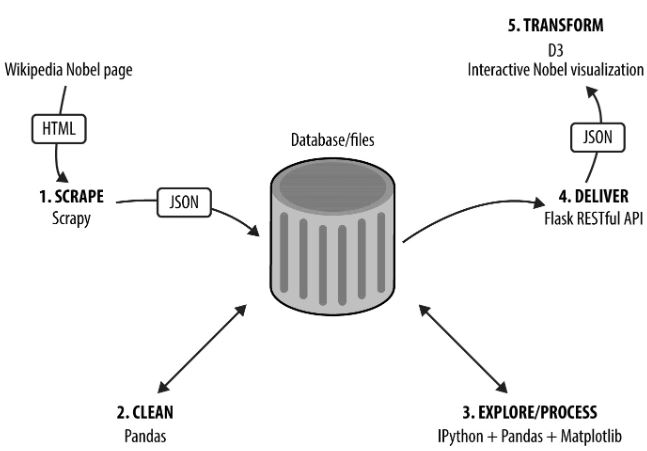
\includegraphics{C:/Users/Katie/OneDrive/Uni_Work_Year4/project/Year-4-Project/markdown/chapters/Interviews/toolchain.jpg}
\caption{The Dataviz Toolchain \label{toolchain}}
\end{figure}

When it comes to static visuals, as investigated in this study, two
commonly used tools as the \textit{ggplot2} package in R and the
\textit{matplotlib} library in Python, which are investigated here.

\section{Background on R and Python}

R and Python are two languages that differ in programming paradigms,
with R being a mostly functional language and Python taking more of a
multi-paradigm approach, incorporating mainly elements of
object-oriented programming, but along with some elements of
procedure-oriented and functional paradigms (Bhaiya
\protect\hyperlink{ref-paradigm}{2020}).

At a basic level, functional programming does exactly what the name
says; it operates mainly using functions to obtain results and output,
with the ability to use certain functions within others to create new
composite functions.

Object-oriented programming, on the other hand, focuses on storing
information in `objects', with attributes as defined by their `class'.
Information in a class structure is then accessed in the format
`class.object'. In addition to objects, `methods', or functions, can be
defined within a class.

These two differing methods of programming, like everything, have a
series of positives and negatives. A positive shared by both R and
Python is that they are open-source, unlike languages such as SAS or
MATLAB, meaning anyone can gain access with no paywalls, and anyone can
contribute to development of new packages and libraries, creating
communities among people who develop in these languages and allowing
creativity of people from all areas to be used in development. Both of
these are also fairly good for creating visualisations in a reproducable
and replicable way due to their programmatic nature.

Some differences between the two languages are outlined by Team
(\protect\hyperlink{ref-rvpy}{2021}). One main difference is R's main
purpose of data exploration and statistical analysis, as compared to
Python use in more general programming, but with applications in data
wrangling. Both therefore can be used for data cleaning, analysis and
visualisation, but R is more suited than Python to running in depth
statistical testing and analysis, whereas Python is more suited than R
to applications such as large-scale machine learning.

These differences are reflected in the visualisation capabilities of
each language; with a focus in data exploration, R comes with the
pre-installed plotting library \textit{graphics}, whereas the more
general programming-based Python must use external libraries.
Additionally to the default library, R can also install
\textit{'ggplot2'}, a library dedicated to producing elegant visuals
with ease.

Python is regarded as a fairly easy to learn language and is known as
one of the most popular languages worldwide, especially among
programmers and developers. R appears to be noted as a generally
slightly more difficult to learn language, but is a popular choice among
statisticians and data scientists, particularly in R\&D.

\subsection{The Grammar of Graphics}

First introduced by Leland Wilkinson in his 1999 book ``The Grammar of
Graphics'' (Wilkinson \protect\hyperlink{ref-wilkinson2009}{1999}), the
`grammar of graphics' is explained by Hadley Wickham in the 2010 paper
\textit{A Layered Grammar of Graphics} (Wickham
\protect\hyperlink{ref-layered-grammar}{2010}) as a method to describe
the underlying components of a visualisation.

It works on breaking every plot into a layers of graphic components,
building visualisations in a systematic way from the ground up. The
first layer consists of the data and a basic aesthetic mapping, with
subsequent layers being made up of components such as scales, coordinate
systems, positioning and geometric objects. Each component, or layer, of
a layered graphic can be considered as independent in this framework,
with each being able to be modified without altering any other
component.

This concept allows effective visualisations to be built in an efficient
way, ensuring all important aspects of a visualisation are considered
and accounted for, as opposed to randomly assigning aesthetics to a
figure on a `trial and error' basis. It allows for the creation of
figures that are bespoke to each problem, with every small element of a
plot being fully under control of the designer.

The transition to learning a grammatical programming system such as
\textit{ggplot} or \textit{matplotlib} from using a software using a
stock library of graphics with tweak-able elements is described by the
author as akin to transitioning to learning \latex after using MS Word.
His reasoning is that it encompasses the initial frustration and feeling
of lack of control over `low-level aspects', but the eventual freedom of
being more deep content focused, leading in the case of plots to
creating `richer graphics much more easily'.

\subsection{Visualising with \textit{ggplot2}}

As mentioned prior \textit{ggplot2} is an R package dedicated to
providing an easy way to produce elegant but complex visualisations,
with applications in simple to complex data analysis and statistics
along with areas such as machine learning.

This package is built to operate in a way that strongly follows the the
grammar of graphics (Wickham \protect\hyperlink{ref-ggplot2}{2011}),
perhaps expected given that the author of
\textit{A Layered Grammar of Graphics} is Harvey Wickham, referenced
prior as the creator of this package. This can be clearly seen in the
structure of commands for creating plots in this package; the first step
in creating a plot in this package is to specify a data frame and
specify an aesthetic mapping using the \texttt{aes()} argument.

After these have been specified, the user ends the line with a
\texttt{+}, which dictates the addition of the next line, which will
comprise of one of the higher level layers to the base layer aesthetic
mapping. It can take some time to learn this format, but becomes
intuitive once the user has an understanding of the concept of the
grammar of graphics, even if they have not explicitly learned it or
heard of this term, and rather have picked it up through practice.

\textit{ggplot2} has the capacity to create complex visuals while
staying informative and retaining aesthetic appeal, and in the right
hands can be an incredibly powerful tool for visualisation of data.

\subsection{Visualising with \textit{matplotlib}}

\textit{Matplotlib} is a Python plotting library that allows the user to
create MATLAB-like visuals while being free and open-source.

There exist two Application programming interfaces (APIs) for the
creation of plots in \textit{matplotlib}; the object oriented interface
of base \textit{matplotlib} and the more functional \textit{pyplot}.
Explained by Sanap (\protect\hyperlink{ref-matplotblog}{2020}), both
interfaces seem to provide effective ways to create elegant and
informative visuals, with the main differences being that
\textit{pyplot} structures the building of visuals in a very similar way
to MATLAB in terms of syntax and methodology.

Both APIs follow the grammar of graphics, with the initial step in
visualisation being the creation of a blank plot to which various
graphic features can be added sequentially.

This method of plotting, like R, provides a very good way to produce
visuals, however unlike R does not specialise in visualisation and
relies on imports and collaborations with other languages, such as
MATLAB and JavaScript. The combination of Python with these other
languages, however, provides very effective methods of producing
compelling visuals, and again can be a very powerful tool.

\chapter{Data collection}

\section{Background on survey design}

As explained by Wiley-Interscience
(\protect\hyperlink{ref-wiley2004}{2004}), a survey is a means of
obtaining quantitative information regarding opinions and experiences of
the respondents in order to explore the views of the target population
as a whole. In this book, a survey is noted as a ``systematic'' method
of collecting data, where the author states that the word ``systematic''
is deliberately used in order to separate surveys from other methods of
information collection. ``systematic'' is defined by the Collins English
Dictionary as something that
\textit{"is done according to a fixed plan, in a thorough and efficient way"}
(Collins \protect\hyperlink{ref-collins-systematic}{n.d.}), and this
reflects the manner in which surveys are created in accordance with a
given system, where methods for distribution, implementation and
analysis are defined under a pre-determined structure. The survey will
be delivered to potential respondents in the target population, who will
then be asked to complete a series of standardised questions, or
questions for which the question ordering and wording is identical for
every respondent, unless different formats are to be used to research
purposes. It is once again discussed by Wiley-Interscience
(\protect\hyperlink{ref-wiley2004}{2004}) that standardised questioning
was not always the norm; most interviewers would more likely have a list
of objectives, and each interviewer would formulate and word questions
based around these. It was discovered that question wording can have a
drastic effect on respondents' answers.

Whether or not the survey is `thorough' and `efficient' depends heavily
on the survey structure and design. Designing an effective, systematic
survey involves balancing efficiency with completeness, creating a
survey that can obtain as much information as possible whilst not boring
or fatiguing participants, which can lead to non-response and
measurement errors due to participants skipping questions or selecting
answers at random. A well-designed systematic survey has the capacity to
yield large amounts of both qualitative and quantitative information
regarding the research topic while minimising these errors.

There exist a variety of methods for delivering a survey, such as
self-completed questionnaires and interviewer-administered interviews.
Depending on the aims of the study, there will be advantages and
disadvantages to each method. There may also be times when a combined
approach is helpful in gathering the necessary information. The first
method of surveying, a questionnaire, may consist of either physical
paper forms that are mailed or handed out to people within the target
population, or in an online format. As discussed by Brace
(\protect\hyperlink{ref-brace2004}{2004}), this form of surveying
constitutes a method of indirect communication between the respondent
and researcher, in effect a non-verbal conversation in which the
respondent is replying to the researcher's questions. The
non-face-to-face aspect of this method can be beneficial in terms of
anonymity; an anonymous respondent is more likely to be honest in their
answers than a respondent for whom the identity is known. As a result,
an anonymous questionnaire can mitigate errors that may be caused by
respondents fearing judgment of their answers. It is also possible to
administer a large number of these questionnaires in a short period of
time since they are self-administered, and thus constraints such as the
number of interviewers or time taken to administer the survey has less
effect on the amount of information obtained.

There are, however negatives to this questionnaire method. In his book,
Brace discusses the way in which question wording must be very carefully
thought about when using this method of indirect conversation, for
reasons such as there being no way to correct participant
misunderstanding of questions. Additionally, the fact that the
researcher and participant never come into contact may allow the
researcher to write questions without considering the human nature of
the participants; it is easy to become absorbed in attempting to gather
information and fall into forgetting that long-winded or complicated
questions may bore or confuse respondents, leading to poorer quality
responses. Similarly including too many questions in the questionnaire
may lead to response errors for the same reasons. It is then crucial to
be as clear and concise as possible in question wording, leaving little
room for interpretation. This type of survey is also a very static
medium; it does not allow for much expansion on participants' answers,
with reasoning behind answers unknown unless specifically requested,
which again could add to respondent fatigue and affect quality of
response.

We can attempt to implement some dynamic discussion into a questionnaire
in the form of `open-ended questions', mentioned above as specifically
requesting reasoning behind answers. A questionnaire is composed of two
types of questions; closed-ended questions, for which the respondent
selects their answer from a given set of potential responses, and
open-ended questions, in which the participants are able to write their
answers in a free-form format. Closed-ended questions are very good for
obtaining quantitative data that may be easily categorised and counted,
which is useful for gathering empirical evidence in order to form
objective conclusions regarding the sample population.

Open-ended questions are generally used where more expansion may be
required in addition to the closed-form answer, or if using a
closed-form question would limit the answer range. The Leibniz Institute
for the Social Sciences (Züll \protect\hyperlink{ref-leibniz}{2016})
provides guidance on open-ended questions, in which the occasions for
using open-ended questions are outlined as:

\begin{itemize}
   \item "knowledge measurement"; with with multiple choice, respondents would have a chance of guessing the correct answer, and thus this would be a sub-optimal way to measure raw knowledge
   \item "Unknown range of possible answers"; multiple choice may be limiting for certain questions, and may cause the researcher to miss important information 
   \item "Avoidance of excessively long lists of response options"; if there is a known range of answers, but this range is very large, it may overwhelm respondents to see all of these as options
   \item "Avoidance of directive questions"; certain questions may have options based on the researcher's own opinions, and thus have the potential to direct the participant in a certain direction, and may not reflect the participants' true views. This links to "unknown range of answers" in that the researcher may incorrectly assume the potential range of answers and thus the given options may not cover the respondents' true opinions.
   \item "Cognitive pretesting", which covers instances such as ensuring the question was understood correctly.
\end{itemize}

To summarise, open-ended questions are useful when either there is not
enough information to set a standardised range of potential responses or
if more information is needed after a closed-ended response.

A method of surveying that is, by design, more dynamic is an interview.
An interview may be structured, semi-structured or structured and each
of these have a different set of features that distinguish them from one
another. Structured interviews, as by the name, are rigid in nature and
comprise of a vocal conversation in which the interviewer has a specific
set of questions from which the discussion does not deviate. The
slightly less rigid semi-structured interview is similar, but slight
deviation from the plan is allowed in order to explore new avenues and
ideas that might not be found with a structured interview, but the
interviewer will still have a set of specific questions for which to
obtain responses. For the most flexible of the three, the unstructured
interview, the interviewer will tend to follow a loose plan of what they
wish to explore rather than a strict question schedule, with the
discussion led by the respondent's answers.

Phone calls and other forms of interview-based survey allow the
interviewer to form a personal connection with the survey participant,
which can be especially helpful for a company's image if the interviewer
is particularly professional or charismatic. Additionally, while the
interviewer will still be limited to asking the pre-set questions, the
format of such a survey can be considered semi-structured and with much
more room for interpretation. This can lend itself to gaining additional
insights that may not have otherwise been gathered from a more
closed-form paper or online survey. Additionally, the more open format
can negate any error as a result of participants misinterpreting
questions due to the interviewer's ability to immediately clarify on any
misunderstandings. This type of survey also provides an instant
response, which is beneficial if there is only a short time frame
available in which to gather information.

However, there are also shortfalls to an interview-based survey method.
For instance, although a charismatic interviewer can positively impact
the image of whoever is conducting the survey, this could also lead to
biases, such as the respondent answering in a way they feel will please
the interviewer. Additionally, the image of the organisation could
potentially be tainted if the interviewer appears rude or
unprofessional, alongside potentially providing bias in the opposite
direction. As well as this, telephone surveys are likely to be
interpreted as a telemarketing scheme, and thus potentially have a
negative impact on the number of willing respondents. The reduced
anonymity of this type of survey may also create bias in the way of
participants avoiding making statements that could be deemed socially
unacceptable, or that they feel they may be judged for, and therefore
may not provide answers accurate to their true line of thought.

The UK Household Longitudinal Study (``Understanding Society - the Uk
Household Longitudinal Study,''
\protect\hyperlink{ref-longitudinal}{n.d.}) is an ongoing study and an
example of implementation of a combined use of the above mentioned
surveying methods. Initially, in `wave 1' of the study, a sample of
40,000 households in the UK were selected to be surveyed on a yearly
basis. The survey involves all members of each selected household,
overall comprising of around 100,000 individuals, and asks them a range
of questions regarding areas such as family life, income, employment and
health. The study consists of a self-administered youth paper
questionnaire given to respondents ages 10-15, and an interview for
those aged 16 and up. This split in age demographic allows some
questions to be omitted from the youth survey, such as those about
income and employment, and some to be added such as about pocket money
habits and `future intentions', as the website states. Giving the youth
respondents a paper questionnaire may help obtain more useful or
relevant answers, as the respondent may be more comfortable with this
than being interviewed by an adult. The youth questionnaire is also
shorter, which could perhaps just be a result of many questions not
being relevant to this demographic, or it could be a conscious decision,
but either way this with help to ensure the young respondent doesn't
lose interest and potentially incur bias in their answers due to either
rushing to finish the survey or not paying attention. The adult survey
also includes a section specific to 16-21 year olds. The surveys contain
a standardised set of core questions asked each year alongside a set
asked every other year. The reasoning behind this is given to be that
this study has a very large scope, asking about many aspects of each
respondents' life, and so it becomes inefficient and counterproductive
to include all questions every year since, as mentioned previously, the
longer a survey is, the more likely a respondent is to get bored or
mentally fatigued. The fact that the adult survey is administered in an
interview also means that there may be limits on the amount of time the
survey can take, as interviewers may have to get through a certain
number of respondents in a day, additionally to the interviewer
potentially also becoming fatigued. If the interviewer is fatigued,
their tone and how they hold themselves may change, and potentially
cause a subconscious bias in how the respondent answers the questions.

\section{Specific goals of survey tool for this study}

While visualisations can be a very useful tool for understanding data,
they also have the potential to be highly misleading. This section of
the study will explore how modifying certain aesthetic features of
visualisations can impact perception and interpretation of data, and how
these modifications can be exploited in order to mislead the observer.
Misleading visualisations may be created in an effort to deliberately
influence the viewers' perceptions, or accidentally as a result of poor
practice and knowledge surrounding data visualisation. In either case,
visualisations have the ability to communicate different messages and
stories depending on how they present the data to the observer.

The specific aim of the survey is to test whether altering y-axis
scaling, bar width, bar grouping method and colouring will have an
impact on single data value interpretation and subjective interpretation
of differences in data values.

\section{Survey Design}

The survey design will be inspired by the papers discussed in the
previous literature review, all of which investigate how different
aesthetic and design choices have the potential to mislead the observer
or alter perception.

Following this, questions included in part 1 the survey will focus on
gauging whether altering the y-scale to be truncated or logarithmic has
an effect on user perception of difference in data point values, for
both bar and line plots. The respondents will be asked to gauge both
individual values and differences in values, with the former providing
an open answer box in which the may type their answer to allow for
maximum freedom and obtain their true observation, unimpeded by the bias
of having a specific set of numbers to pick from when their true
observation may lie outside this range. The question for gauging
difference perception follows Lauer and O'Brien
(\protect\hyperlink{ref-claire-obrian}{2020}) and Yang et al.
(\protect\hyperlink{ref-YANG2021}{2021}) in using a numbered scale with
numbers representing a range from not much difference up to a large
difference. The Yang et al. (\protect\hyperlink{ref-YANG2021}{2021})
method of a 7-point scale was employed here. From these papers, it is
hypothesised that the truncated scale will cause respondents to
overestimate differences between data values, and the logarithmic scale
will be hypothesised to result in underestimation.

Additionally, stacked bar charts will be investigated, showing a
comparison between using the stacking method as opposed to a grouped bar
plot. Based on reviewing the literature, part 3 of the survey will
include questions with the objective of testing standard stacked against
grouped bar charts, alongside questions relating to the colour palettes
used in depicting the different groups. We aim to test which colour
palette is preferred in terms of aesthetics as well as ease of
interpretation and reading.

The last two parts of the survey, noted henceforth as `Sales - part 1'
and `Sales - part 2', explore the different y-axis scalings with respect
to line plots, but for these, as opposed to the bar plots, the default
was a truncated axis. The three plots investigated will consist of line
plots relating to time series data for two fictitious companies. One
will display each of the two lines on separate plots with the default
axis, one will show both on the same plot with the default axis, and
finally one with both on the same plot but with a zeroed axis. It is
hypothesised that a difference in value for two time points will be
perceived as smaller fopr the zeroed axis, and larger for the separated
plots.

As discussed in Peytchev and Peytcheva
(\protect\hyperlink{ref-Peytchev_Peytcheva_2017}{2017}), too long a
survey can result in higher measurement error due to factors such as
waning interest or mental fatigue of respondents, resulting in careless
responding and non-response. This is also further explored in Brower
(\protect\hyperlink{ref-brower}{2018}), whereby a study is carried out
to determine causes of careless responding, and specifically looks at
questionnaire length and participant disinterest. The study performed in
this work provides evidence that longer survey length can have a
detrimental affect on careless responding; a long survey may make
participants more likely to respond carelessly, and this must be
considered when designing an effective and efficient survey. An
additional conclusion states that participant interest in the survey
content could have an effect, but also that evidence is less supported
for this claim. There is significant enough evidence, however, to say
that this should also be considered when designing the survey.

The Peytchev and Peytcheva
(\protect\hyperlink{ref-Peytchev_Peytcheva_2017}{2017}) paper explains
that a `split survey' design, where each respondent is only asked to
answer a selection of questions from the whole set, is effective in
reducing error while gathering large amount of information, however this
will not be employed here. The reasoning for this is that there will
already be a set of 12 different surveys being sent, and creating
further splits could potentially lead to much too small sample sizes and
thus inconclusive results. Additionally to this, the paper investigates
how placement of questions in the survey can affect responses,
concluding that questions asked later in the survey are more susceptible
to bias, which tracks with the conclusion of survey length being a cause
of careless responding; the longer a participant is taking a survey for,
the more likely they are to start being careless with responding.

Due to this, the survey was designed to last in the range of
approximately 15-20 minutes, as suggested in Revilla and Ochoa
(\protect\hyperlink{ref-length}{2017}). One paper (Crawford, Couper, and
Lamias \protect\hyperlink{ref-burdenpercep}{2001}) explores the pecieved
burden of a survey on the participant, and performs a study whereby
respondents were assigned a questionnaire, but given one of two
different time estimates, for which the true length of the survey lay
between. It was found that more people started the survey with the lower
estimated completion time, but more also dropped out. However, the time
at which respondents dropped out did not significantly differ in the two
groups. In order to obtain maximum response, it is wise to as accurately
as possible disclose the true survey length, and even slightly
over-estimate in the disclosure.

With regard to the interest factor, the survey was designed with
engaging respondents. The topic of the majority of the survey was chosen
to be data relating to the television show
\textit{American Ninja Warrior}, as this could be subjectively viewed as
a `more interesting' topic than seemingly meaningless numbers. The
survey was administered to a test subject, who commented that they found
this topic interesting, with the additional comment that perhaps some
pictures of the Ninja Warrior obstacles would be nice, however was not
employed. The survey also took this respondent about 20 minutes to
complete.

Although the content of the surveys for this study is not likely to be
controversial or highly personal, anonymity is still important as the
participants could otherwise potentially feel pressure to give a
`correct' answer, given the mathematical nature of the questions. As
mentioned prior, anonymity here means that this pressure is potentially
reduced and thus the relevant measurement bias may be mitigated.
Additionally to the more technical visualisation questions, respondents
were asked a series of demographic questions such as age, degree subject
(if applicable), and whether they are colourblind or have any disorders
that my affect visual processing. Additionally, three Likert scaled
questions relating to well they would rate their spatial, observational
and numerical skills. The Yang et al.
(\protect\hyperlink{ref-YANG2021}{2021}) paper, which explores the
truncation effect of barplots, looks at graph literacy and its relation
to perception, and hypothesises that those undertaking quantitative
subjects at PhD level would be less impacted by the truncation effect as
compared to humanities PhD students. It was found that the truncation
effect did impact both groups, but those in quantitative fields had
their perception marginally less affected. Thus the degree subject
question was included to explore if this has an effect here. In relation
to the visual processing and colorblindness questions, these are again
included to test whether they have any significant impact on perception,
as it may be important to consider these factors when creating
visualisations to ensure they are accessible to all, and the study will
examine the potential impact of such disorders.

The set will consist of two groups of surveys, which will be identical
up to the visualisation package used. Particularly, one group will
contain visualisations made with R's ggplot2, the next with matplotlib
from Python. These surveys will be distributed to the general public by
sharing links on social media platforms such as Facebook. The reasoning
behind creating two separate surveys in different languages is to
ascertain whether the language used influences the interpretation.
Within the groups there are 6 surveys, with each altering the order of
visualisations shown in part 1 to assess the perception of each plot
type without reference or comparison to another, and the same with part
2. in Part 3, each of the 6 used one of 3 colour palettes as the main
colour, and another as a comparitor to test which the preferred colour
palette is and which respondents find easier to read and interpret. Note
however that, while both languages were intended to be as close to
default as possible, the ggplot visualisations were made such that the
theme \texttt{theme\_classic} was applied, as this is mirrors the Python
format in terms of the absence of grid lines. Thus any comparisons made
are to be considered as be comparing standard matplotlib and ggplot with
the classic theme.

\section{Creating the Visualisations}

See appendix 1 for a pdf of the survey, containing the finished visuals,
and appendices 2 and 3 for code.

\subsection{The Data}

The visualisations for the survey were created with inspiration from the
papers discussed above. The bar plots were created using a data set
regarding the history of obstacles used over 10 seasons of
\textit{'American Ninja Warrior'} (see LAESSIG,
\protect\hyperlink{ref-ANW}{n.d.}). Each row of the data represents a
single instance of an obstacle being used, and each instance has
variables as specified in table 2.1.

\begin{center}
\begin{table}

\caption{\label{tab:unnamed-chunk-4}Table with explanation of variables}
\centering
\begin{tabular}[t]{l|l}
\hline
Variable Name & Explanation\\
\hline
season & Season in which instance occured\\
\hline
location & Location of use\\
\hline
round\_stage & Stage of competition in which instance occured\\
\hline
obstacle\_name & Name of the obstacle\\
\hline
obstacle\_order & Order in which the obstacle was placed in the course\\
\hline
\end{tabular}
\end{table}
\end{center}

This data was manipulated in R to produce a data frame containing the
count of the number of times each obstacle was used over the course of
the whole ten seasons. For the stacked and grouped bar plots, a data
frame was produced, once again in R, containing columns `obstacle' and
`stage', where `obstacle' is a vector containing the name of each
obstacle repeated the number of times it was used, and `stage' similarly
contains the names of all the stages of the competition, with each
repeated the number of times it appeared. For example, Salmon Ladder was
used 41 times, and thus is also repeated this many times, and there are
41 entries in the `stage' vector corresponding to this. For the python
version, the frequency tables were created manually.

The data for the time series plots was taken from the data set
\texttt{BJsales} in the base R package \texttt{datasets} (R Core Team
\protect\hyperlink{ref-R}{2017}). This data consists of a single vector
of values with 150 entries, where each entry corresponds to a
measurement taken at some arbitrary time point. Four subsets were taken
from this data such that a start index was selected, and then this entry
and the 11 following consecutive entries were extracted. The vectors
were put into a data frame with the time steps set as months, giving a
year of sales data for four fictional companies. This again was used to
manually create a data frame in Python. To select the starting index,
several seeds were tested for random selection, and four seeds were
selected that would create plots to best test the hypotheses.

\subsection{The Bar Plots}

As explained before, the bar plots for part 1 were made such that one
uses the default axis scaling, one uses a truncated axis, and one uses a
logarithmically-scaled axis. It is worth noting that in R attempting to
truncate the bar plot itself does not work; the bar must start at the
zero tick mark otherwise the bars do not show up. To get around this
issue, the data itself was truncated before applying to a bar plot with
the tick labels then altered to fit the truncation, using intervals of
10 as in the default plot. Python, on the other had, will perform the
truncation without this issue and defaults to steps of 2.5, which could
affect the reading of values. For the logarithmically scaled plots, R by
default starts at 1 and uses a non-standard form notation with tick
labels of 1, 3, 20, 30. Python does use standard form and has labels 0,
\(10^0\) and \(10^1\), starting at zero. The Python scale starting at
zero was before mentioned as potentially misrepresenting the data. The
height gauging of the R plot could maybe be impacted by the scale
starting at 1. The default for the Python control plot scaling was more
granular than the R, with steps on 5 as opposed to 10. The control
scales for both languages have a range {[}0, 40{]}, and {[}20, 40{]} for
the truncated plots. There were 4 bars corresponding to 4 of the most
used obstacles, arranged in descending order.

The next part plays with the aspect ratio of the plots. In order to keep
this accurate, the plots were saved within the code as opposed to saving
from the viewing window. The default aspect ratio for the ggplot is 1/1
for height to width, and using pyplot.gca() and comparing to the default
we see that the default for Python using this method is 0.1. For the
`wide' plot, the aspect ratios are halved to 0.5/1 and 0.05,
respectively. For the narrow, the aspect ratios were doubled to 2/1 and
0.2. Note that the aspect ratios include the entire plotting area,
including labels and titles. These plots contained 7 bars as opposed to
the 4, but were still arranged in decending order.

The plots in the third part of the survey were the stacked and grouped
plots. The three colour schemes were the package default, a greyscale,
and the colurblind-friendly Viridis palette (Garnier
\protect\hyperlink{ref-viridis}{2018}). The obstacles here were the same
4 as displayed in part 1, but with the added colours for the competition
rounds. The default axis ratios here mean that the R plots appear taller
in comparison to their width than the Python plots, due to the legends.

\subsection{The Line Plots}

The plots for part 1 of this show the false sales data in the form of
time series line plots, where the x-axis displays the months and y-axis
shows number of sales. In the R version, the x-axis displays the 12
months in words, whereas the x-axis of Python version numbers the months
and plots them in intervals of 2 months. This was an unintentional error
on the part of the designer, however could be used to draw conclusions
regarding how the two systems differ; monthly ticks in words or
bi-monthly numbers. The plots in sales- part 2 were created very
similarly, just with two different start indices.

\section{The Survey}

This section will discuss the specific survey questions and explain the
differences in plot ordering and colour schemes between survey versions.
Google forms was chosen as the medium for delivering the survey, as it
is a free service and provides easy way to send out survey links and
automatically compiles responses in a Google sheet along with time
stamps, which can be exported to csv for analysis. To randomly assign
each participant a survey, a javascript code was created to link to a
landing page, which redirected the participant randomly to one of the 12
surveys. As time progressed it was possible to see how many respondents
were taking each survey, and it was possibly to alter the Javascript
accordingly to ensure each survey had an approximately even number of
respondents. The survey was set such that each page contained a single
question with a set of related sub-questions and only the plots relevant
to these sub-questions, to prevent participants scrolling through the
survey and seeing other figures which may alter their perception. This
can also be used to analyse the effect of seeing other plots on
perception of the plots following.

\subsection{Demographic Questions}

As discussed, the questions below are used to assess whether these
factors have an impact on graph literacy and graph perception.

\begin{itemize}
    \item Please enter your age (Open)
    \item If you are a university student or past university graduate please specify your area of study. (Drop down box: Science, Technology, Engineering, Maths, Arts, Social Sciences, Humanities, Business, N/A, Other (please specify))
    \item How strongly do you agree with each of the following statements? (Linear scale with 1 - 5, 1=strongly disagree, 5=strongly agree)
    \item  - I have good spatial awareness skills 
    \item  - I have good observational skills 
    \item  - I have good numerical skills 
    \item Are you colourblind? (Checkbox: Yes, No, Prefer not to answer)
    \item Do you have any disorders that may affect visual processing? (this could be a general visual processing disorder 
    or dyslexia, dyscalculia, ADHD etc)
    ((Checkbox: Yes, No, Prefer not to answer))
\end{itemize}

\subsection{American Ninja Warrior - Part 1}

The questions regarding each of the three bar plots were as follows:

\begin{itemize}
  \item Approximately many times would you say the 'Salmon Ladder' was used? (Open)
  \item Approximately how much more than 'Log Grip' would you say 'Salmon Ladder' was used? (1-7 scale)
  \item Approximately how much more than 'Quintuple Steps' would you say 'Salmon Ladder' was used? (1-7 scale)
  \item In your opinion, approximately how many times would you say 'Log Grip' was used, as a percentage of the number of times 'Salmon Ladder' was used? (Open)
\end{itemize}

Here, the two questions with the difference rating scale are used to
assess whether having the bars next to each other vs on opposite ends of
the plot has an effect on the difference in rating when comparing the
responses for each of the plots. The use of the word `more' in these
questions could perhaps be considered leading, as it indicates to the
respondent the direction of the difference. The wording of part 2,
specifying that distance is being compared but without specifying a
direction, may have been better here, and next time would be used.
However, this is unlikely to have has too large of an effect, as it is
easy to see that the `Salmon Ladder' was used most out of the four
obstacles.

Question 4 here was perhaps too wordy and/or confusing, and asks
effectively the same question as the two previous. If this survey were
to be applied again, this would be omitted as it adds unnecessary
respondent fatigue. This is especially the case since the responses to
this question mean it has been omitted from analysis, and so added to
respondent fatigue without any additional information gain.

The table below shows all the permutations of the three plot types, and
which questionnaire version they appear in.

\begin{center}
\begin{table}

\caption{\label{tab:unnamed-chunk-5}Order of plots in part 1}
\centering
\begin{tabular}[t]{l|l|l|l}
\hline
  & Q1 & Q2 & Q3\\
\hline
V1 & Control & Log & Truncated\\
\hline
V2 & Control & Truncated & Log\\
\hline
V3 & Log & Control & Truncated\\
\hline
V4 & Log & Truncated & Control\\
\hline
V5 & Truncated & Control & Log\\
\hline
V6 & Truncated & Log & Control\\
\hline
\end{tabular}
\end{table}
\end{center}

The table shows that, for example, in version 1, the control plot was
shown in question 1, the log-scaled in question 2 and the truncated in
question 3.

\subsection{American Ninja Warrior - Part 2}

The questions regarding each of the three bar plots were as follows:

\begin{itemize}
  \item How large would you say the difference between 'Jumping spider' and 'Salmon Ladder' is? (1-7 scale)
  \item How large would you say the difference between 'Log Grip' and 'Floating Steps' is? (1-7 scale)
  \item How many times would you say 'Floating Steps' were used? (Open)
\end{itemize}

In hindsight, the value judgment question should perhaps have used the
same phrasing as part 1. Removing the word `approximately' from the
value judgment question could have an adverse affect on responses by
comparison to part one in the way of perhaps making respondents feel
they have to give a more `accurate' and less subjective response than
part 1.

Similar to part 1, the below table gives all permutations of the three
plot types.

\begin{center}
\begin{table}

\caption{\label{tab:unnamed-chunk-6}Order of plots in part 2}
\centering
\begin{tabular}[t]{l|l|l|l}
\hline
  & Q1 & Q2 & Q3\\
\hline
V1 & Default & Narrow & Wide\\
\hline
V2 & Default & Wide & Narrow\\
\hline
V3 & Narrow & Default & Wide\\
\hline
V4 & Narrow & Wide & Default\\
\hline
V5 & Wide & Default & Narrow\\
\hline
V6 & Wide & Narrow & Default\\
\hline
\end{tabular}
\end{table}
\end{center}

Questions regarding comparisons between the plots were then administered
as follows, while showing respondents all of the three plots on a single
page.

\begin{itemize}
  \item Which of the three bar charts do you find most aesthetically pleasing? (Multiple choice with options "A", "B" or "C")
  \item Which bar chart do you feel is easiest to read and interpret? (Multiple choice with options "A", "B" or "C")
  \item Which bar chart do you find hardest to read and interpret? (Multiple choice with options "A", "B" or "C")
\end{itemize}

\subsection{American Ninja Warrior - Part 3}

This part explored the differences in perception for stacked and grouped
bar charts, alongside colour preferences. This part had 4 questions,
with the first two asking about the stacked and grouped bar plots, with
either the stacked first or grouped first.

The first two sub-questions are given below.

\begin{itemize}
  \item How many times would you say 'Floating Steps' were used in the Finals (Regional/City) rounds? (Open)
  \item How many times would you say 'Log Grip' was used in the Finals (Regional/City) rounds? (Open)
\end{itemize}

The next question is ``Please select the statement you feel applies to
the bar chart above.'' and consists of a multiple choice answer with the
following options:

\begin{itemize}
  \item 'Log Grip' was used MORE in Finals (Regional/City) rounds than in Qualifying (Regional/City) rounds.
  \item 'Log Grip' was used Less in Finals (Regional/City) rounds than in Qualifying (Regional/City) rounds. 
  \item 'Log Grip' was used an EQUAL number of times in Finals (Regional/City) rounds and Qualifying (Regional/City) rounds.")
\end{itemize}

This is followed by another multiple choice question, given as Which
obstacle do you think was used MORE in Finals (Regional/City) rounds,
`Log Grip' or `Floating Steps'?, with the following options:

\begin{itemize}  
  \item 'Log Grip'
  \item 'Floating Steps'
  \item They were used the same amount of times
\end{itemize}

After answering these questions for both plot types, the respondents
were shown both on the same page and asked to select which of the two
they found easier to read and interpret, and were then shown the stacked
bar plot in two different colour palettes; the one used for the
questions so far and a comparitor, with the questions below.

For the stacked vs grouped comparison:

\begin{itemize}
  \item Which bar chart do you feel is easiest to read and interpret? (Multiple choice with options "A", "B", "C")
\end{itemize}

For the colours comparison:

\begin{itemize}
  \item Which colour scheme do you find most aesthetically pleasing? (Multiple choice with options "A", "B", "C")
  \item Do you feel that one of the colour schemes makes it easier to read and interpret the data than the other? If so, please select which one. (Multiple choice with options "No", "Yes, A is easier", "Yes, B is easier")
\end{itemize}

For this part, survey versions 1, 2 and 4 showed the stacked bars first,
followed by the grouped, and versions 3, 5 and 6 displayed the grouped
first. It is shown in the below table which colour schemes were used in
each survey.

\begin{center}
\begin{table}

\caption{\label{tab:unnamed-chunk-7}Colour palette pairings used in each question}
\centering
\begin{tabular}[t]{l|l|l}
\hline
Version & Main colours & Comparitor\\
\hline
V1 & Viridis & Default\\
\hline
V2 & Default & Viridis\\
\hline
V3 & Default & Greyscale\\
\hline
V4 & Greyscale & Default\\
\hline
V5 & Viridis & Greyscale\\
\hline
V6 & Greyscale & Viridis\\
\hline
\end{tabular}
\end{table}
\end{center}

\subsection{Sales - Part 1}

The respondents then moved onto part 1 of the sales section of the
survey, in which they are asked to once again give subjective opinions
regarding the y-axis scaling, but this time relating to time series line
plots.

Once again, the same set of questions is asked for each plot which
consist of, firstly, a two-row multiple choice grid, with each row
relating to one of the companies. Respondents were asked the question
``How much would you say sales of each company increased between January
and December?'' and were to give a response on the 7-point scale. Again,
this could be seen as leading due to the word ``increased'', and in
hindsight this could be altered to read ``changed'', with the response
options then potentially on a scale with the centre value (ie 4 on a 7
point scale) corresponding to no change, and the numbers on either side
representing a positive or negative change. This would also perhaps be
implemented in the questions regarding comparisons of bar heights.

The ordering of the plots for each version number are given below.

\begin{center}
\begin{table}

\caption{\label{tab:unnamed-chunk-8}Order of plots in part 3}
\centering
\begin{tabular}[t]{l|l|l|l}
\hline
  & Q1 & Q2 & Q3\\
\hline
V1 & Separated & Truncated & Zeroed\\
\hline
V2 & Separated & Zeroed & Truncated\\
\hline
V3 & Truncated & Separated & Zeroed\\
\hline
V4 & Truncated & Zeroed & Separated\\
\hline
V5 & Zeroed & Separated & Truncated\\
\hline
V6 & Zeroed & Truncated & Separated\\
\hline
\end{tabular}
\end{table}
\end{center}

The second question was ``How large would you say the drop in sales
between April and July of Company A is?'', which once again was rated
based on the 7-point scale.

\subsection{Sales - Part 2}

The final part of the survey showed zeroed and truncated plots once
again, for two different fictitious companies, this time with the
intention of gaining an overall view. For each of the two, each
respondent was asked a single 7-point scale rating question; ``Based on
the above graph, how large would you say the difference is between the
number of sales Company C makes and the number of sales Company D
makes?''.

\chapter{Univariate Analysis}

This chapter will discuss basic univariate analysis of the survey
results, including summary statistics and univariate testing for the
whole population as well as the subsetting for the programming language
used and degree type. Additionally, subsets will be created considering
only the first plot shown for each question, drawing comparisons between
responses for these plots themselves without influence of the others.
The analysis will be performed in R version R version 4.0.2 (R Core Team
\protect\hyperlink{ref-R}{2017}).

In terms of testing, Shapiro-Wilk tests will be applied with the
\texttt{shapiro.test()} function to gauge whether the data sets can be
considered normally distributed and thus whether parametric T-Tests are
suitable for either one-sample or paired comparisons, for the
Shapiro-Wilk test, the alternative hypothesis is that the data is not
normally distributed. Failing he normality condition, a symmetry test
will be administered via the \texttt{symmetry.test()} function from the
package \texttt{lawstat} (Gastwirth et al.
\protect\hyperlink{ref-lawstat}{2020}), and providing there is
insufficient evidence to reject the null hypothesis that the data is
symmetric, a Mann-Whitney-Wilcoxon (MWW) test will be used. If there is
sufficient evidence that data proves neither symmetric nor normally
distributed, sign tests will be applied. MWW will also be used for two
sample testing where perhaps a sign test would be most appropriate, but
cannot be used as the samples are of different sizes.

The sample sizes are 70, 38 and 32 for the whole population, R subgroup
and Python subgroup, respectively before removing NA of invalid values.
The sample means and medians will be notated as \(\bar{x}\) and
\(\tilde{x}\), respectively.

See appendix 4 for all statistical testing results and p-values.

\section{American Ninja Warrior - Part 1}

This part of the survey assess the effect of truncated and logarithmic
scaling on bar plots perception and interpretation.

The final question in part 1 of the survey,
\textit{'In your opinion, approximately how many times would you say 'Log Grip' was used, as a percentage of the number of times 'Salmon Ladder' was used?'}
will not be considered as it is similar to the previous questions, and
responses ranged in form, between percentages and decimals, and it can
not just be assumed that all the decimals can be converted to
percentages; for example a value of 0.5 could be the decimal value for
\(50\%\), or the respondent could have meant this as \(0.5\%\).

\subsection{Effect of Y-Axis Truncation}

In general, truncating the y-axis had less of an effect than
anticipated. In question 1,
\textit{"Approximately many times would you say the ‘Salmon Ladder’ was used?"},
for which the true value was 41, the distribution of responses for the
truncated plot (\(\bar{x} = 41.35\)) as compared to that of the control
plot responses (\(\bar{x}=41.21\)) shows a small difference, with the
mean perceived value of the bar being slightly higher for the truncated
plot. The median for both of these is 41, showing that both
distributions are centered around the true value of 41. The control and
truncated plots have contextually fairly small variances of 0.752 and
0.753 respectively, depicting both that there is limited variation in
the responses and most of the observations lie fairly close to the
respective means. The variances are also quite similar, showing that the
distributions appear fairly similar, as emphasised by observing figure
3.1 below.

\begin{figure}
\centering
\includegraphics{main_files/figure-latex/unnamed-chunk-11-1.pdf}
\caption{Density plot showing distributions of responses regarding the
control and truncated plots for the question 1}
\end{figure}

Performing a dependent-samples sign test comparing these two sets of
responses confirms that there is no significant difference
(\(p = 0.1877\)) in the response distributions. However, the one sample
sign tests show that there is not sufficient evidence to suggest the
control plot responses differ from the true value of 41
(\(p = 0.1214\)), but there is evidence to accept the hypothesis that
the truncated plot responses differ from the true value
(\(p = 0.0026\)). This shows that, while there is insufficient evidence
from sign testing to suggest a statistically difference in the responses
for the two plots, the location of the truncated plot responses may be
slightly further from the true value than the control, and it is
confirmed by a one sided sign test with an alternative hypothesis that
the true median of truncated responses is greater than 41
(\(p=0.0002\)). This gives evidence that the truncated plot results in a
slight overestimation in reading of the bar height as compared to the
true value of 41. Note that in the responses for the control plot for
question 1, there was a response of ``41/41'', which was taken to be
41.5.

In question 2,
\textit{'Approximately how much more than 'Log Grip' would you say 'Salmon Ladder' was was used?'},
the set of responses for the truncated plot (\(\bar{x} = 5.87\),
\(\tilde{x} = 6\)) is considered significantly different by a
dependent-samples sign test from the control plot responses
(\(\bar{x} = 5.36\), \(\tilde{x} = 5\)). By eye, the average values do
not seem too different between the two plot types, although the p-value
of the sign test (\(p = 0.00019\)) shows that there is in fact a
statistically significant difference. The perceived difference for the
truncated plot being rated higher on average than for the control plot
provides evidence to accept the hypothesis that using a truncated scale
can cause differences in bar height to appear larger, once again this is
confirmed by a one-sided sign test (\(p=9.554e-05\)), with the
alternative hypothesis that the true median of truncated responses is
greater than that of the control responses.

\begin{figure}
\centering
\includegraphics{main_files/figure-latex/unnamed-chunk-13-1.pdf}
\caption{Bar plot showing distributions of responses regarding the
control and truncated plots for question 2}
\end{figure}

The spread for the truncated and control plot responses are slightly
skewed to the right, depicting that the subjective view on the
difference between the bar heights was that it was in general on the
larger side. Looking at the bar heights, for the responses of 4 and 5
the control plot bars are higher, and vice versa for the truncated plot
response bars. This again emphasises the evidence to support the
hypothesis that truncation leads to larger perceived difference.

Question 3 of part 1,
\textit{'Approximately how much more than 'Quintuple Steps' would you say 'Salmon Ladder' was used?'},
asks a similar question to question 2, but asks respondents to judge the
difference for bars on opposite ends of the plot as opposed to next to
each. Again, the by eye comparison shows not a massive difference
between distributions of responses for the control (\(\bar{x}=3.12\),
\(\tilde{x}=3\)) and truncated (\(\bar{x}=3.12\), \(\tilde{x}=3\))
plots, although the sign test shows that the there is evidence to
suggest that the truncated plot responses are in fact on average greater
than for the control plot (\(p=4.624e-06\)). figure 3.3 shows the
distribution of responses.

\begin{figure}
\centering
\includegraphics{main_files/figure-latex/unnamed-chunk-15-1.pdf}
\caption{Bar plot showing distributions of responses regarding the
control and truncated plots for question 3}
\end{figure}

The response distributions, conversely to question 2, now seem skewed
more to the left. However there is a similarity in the way that for the
lower ratings of 2 and 3, the control plot response bars dominate, and
for the responses of 4 and 5 the opposite is true.

Overall, it seems that the use of truncation has a small but
statistically significant effect on perception of height difference
between bars, with respondents tending to judge the difference as
slightly larger than for the control plot, although this effect is
smaller than initially anticipated, and larger for bars that are further
apart. In terms of reading values from bars, the truncation did not have
a statistically significant effect when comparing the two distributions,
however in one sample testing the truncated plot responses did differ
significantly from the true value.

When considering the language subgroups, note that there is a
discrepancy here between languages in terms of the axis tick breaks and
labeling, with the R plot being incremented in steps of 10 for both the
control and truncated plots and the Python being more granular in steps
of 5 for the control and steps of 2.5 for the truncated.

Consider question 1. Comparing the two language subgroups for the
truncated plot, the distributions for both the R (\(\bar{x} = 41.56\),
\(\tilde{x} = 41\)) and Python (\(\bar{x} = 41.01\), \(\tilde{x} = 41\))
responses to question 1 appear similar in location to those of both each
other and the whole population (\(\bar{x} = 41.35\),
\(\tilde{x} = 41\)).

Comparisons via MWW testing show that the responses related to the
control plot differ statistically significantly between the two language
cohorts (\(p=0.00012\)), and similar for the truncated plot responses
(\(p=0.02163\)), where the tests were performed comparing first the R
and Python responses for the control plot, and then for the truncated.

A sign test shows sufficient evidence that the R subgroup responses
relating to the truncated plot differ from the true value
(\(p = 0.0004\)), whereas there is insufficient evidence when applying a
MWW test to the Python responses (\(p = 0.718\)). Similarly, the R
subgroup's responses in relation to the control plot statistically
significantly differ from the true value (\(p=7.629e-05\)), but the
Python subgroup's do not (\(p=0.1185\)). This could potentially be a
result of the less granulated R plot scaling, due to the reduced
precision.

\begin{figure}
\centering
\includegraphics{main_files/figure-latex/unnamed-chunk-17-1.pdf}
\caption{Density plot showing distributions of responses regarding the
control and truncated plots for the question 1}
\end{figure}

The distributions for the control and truncated plot responses for the R
subgroup are fairly similar to the whole population, although the peaks
for the logarithmic plot responses are marginally lower. The
distribution of the truncated plots is unexpected from lokking at the
numbers, and more `chaotic'. This shows potentially more variation in
the responses.

For question 2 it is similarly seen that the language used does not have
a statistically significant impact on the response for the truncated
plot, with means \(5.500\) and \(5.187\), and medians \(6\) and \(5\)
respectively for R and Python for the control plot, and means \(5.98\)
and \(5.84\) both with median \(6\) for the truncated. Comparative
testing with MWW gives \(p=0.2199\) for the control plot and \(0.9105\)
for the truncated. Thus, the scale granulation or any other differing
aspect of the plots does not seem to have a significant effect. See
figure 3.4 for the distributions.

\begin{figure}
\centering
\includegraphics{main_files/figure-latex/unnamed-chunk-19-1.pdf}
\caption{Bar plot showing distributions of responses regarding the
control and truncated plots for question 2, for the R and Python
subgroups}
\end{figure}

For question 3, it is again seen that the responses in relation to the R
version of truncated plot (\(\bar{x} = 3.76\), \(\tilde{x} = 4\)) do not
differ significantly to those related to the Python version
(\(\bar{x} = 3.78\), \(\tilde{x} = 4\)), with a two sample MWW p-value
of 0.9708. Similarly the control plot, there is little difference
between the R (\(\bar{x} = 3.342\), \(\tilde{x} = 3\)) and the Python
(\(\bar{x} = 2.87\), \(\tilde{x} = 3\)) versions of the plot, again with
am MWW p-value 0f 0.1465.

\begin{figure}
\centering
\includegraphics{main_files/figure-latex/unnamed-chunk-21-1.pdf}
\caption{Bar plot showing distributions of responses regarding the
control and truncated plots for question 3, for the R and Python
subgroups}
\end{figure}

Figure 3.4 shows both distributions, with the R appearing more
positively skewed and the python looking fairly symmetric for both plot
types, which was also found when performing symmetry tests. For the
Python it can also easily be seen that the bars for the truncated plot
responses seems `shifted' to the right slightly as compared to the
control.

Now considering subsetting for the respondents that saw the truncated
plot first out of the three. Note that 25 saw the control plot first and
23 saw the truncated plot first.

The distribution of responses for the truncated plot in question 1 shows
a slightly higher mean (\(41.696\)) and median (\(41.25\)) than for the
whole population, but a MWW test shows that the difference is not
significant (\(p=0.1379\)). Similarly for questions 2 and 3, performing
tests on the truncated plot for respondents who saw this first as
compared to the truncated plot responses for the whole population result
in p-values of \(0.2614\) and \(0.3145\), providing evidence that the
plot order doesn't have much of an impact on perception for the
truncated plot.

The conclusions appear to be consistent with results from the Yang et
al. (\protect\hyperlink{ref-YANG2021}{2021}) paper, in which the
researchers, similar to this survey, showed participants a series of
control bar plots alongside those with a truncated axis, and concluded
that the difference in values for the truncated axis were perceived to
be larger than those of the control plots.

\subsection{Effect of Logarithmic Scaling}

Within the logarithmic responses, there were two invalid responses,
given as `Don't know' and `Next to none.'. These will be considered as
`NA' responses and discounted from the quantitative analysis, however
they do provide useful qualitative insights into how the respondents
reacted to the plots, particularly as both were entered for the
logarithmically scaled plot made in Python.

The mean of the responses for the logarithmically-scaled plot, on the
other hand, was magnitudes higher than the true value at 1.493e+13,
although with a median of 35; lower than the median response of the
control and truncated plots responses. The high magnitude is the result
of two answers of `10\^{}15' and `10\^{}9', both again for the python
version of the plot.

The default logarithmic scaling in Python uses standard form notation,
which perhaps the two participants who entered the high magnitude
answers were less exposed to and not as familiar with. Looking at the
degree subjects for these respondents, it is observed that they study
Social Sciences and Psychology, respectively. This could add to the idea
that they are less familiar with this notation as it is more commonly
used in mathematical and physical science disciplines. One of the
respondents also rated their numerical skills at 1/5, showing they feel
that numerical skill is not their specialty. The other rated their
numeric skills at 4/5, showing that even with a good self-perceived
level of numerical skill, standard form could be considered misleading.

This should perhaps be considered when designing visualisations; the
creator of the visualisations may find the logarithmic scale or standard
form more effective in showing the data, but they should consider the
target audience. Are the audience going to be familiar with this? If,
for example, visualisations are being published in a paper targeted at
academics in a subject likely to use such scalings often and understand
them, this may be a good way to depict the data. However, using this in
something such as an advertising campaign could mislead the public,
causing them to either over or under estimate values. As previously
discussed, however, this is often done deliberately in order to push the
message the creator wishes to sell.

The variance in the responses for the logarithmic plot is also high,
with value \(1.492 \times 10^{28}\), showing that a large amount of the
observations differ from the very high mean, and considering this
alongside the lower median may point towards many of the respondents
either giving an accurate response or even underestimating. Furthering
this point, the IQR for the logarithmic responses is the interval
\([30, 40.5]\), which sits below the true value, displaying that over
50\% of the observations in the total population actually underestimate
the value.

The distribution of responses in the R subgroup also shows on average a
slight underestimation (\(\bar{x}= 39.73\), \(\tilde{x} = 35\)) and, as
expected, vast overestimation for the Python version
(\(\bar{x}= 39.73\), \(\tilde{x} = 35\)). This shows that, with a
linearly notated logarithmic scale, the scale may cause underestimation,
but this is counteracted by using a standard form notation.

It can be considered to follow the convention of values that have value
outside the range \([Q1 - 1.5 \times IQR, Q3 + 1.5 \times IQR]\), where
\(Q1\) and \(Q3\) are the first and third quartiles, which here would be
the range \([14.25, 60.75]\) and results in a sample size of 59.
Consider now the response distribution for the logarithmically-scaled
plot, after removing these responses, for which figure 3.7 gives the
density plot. Both plots show the response distribution of the
outlier-removed set of responses, with the providing a comparison with
the distribution of responses relating to the control plot.

\begin{figure}
\centering
\includegraphics{main_files/figure-latex/unnamed-chunk-24-1.pdf}
\caption{Density plot showing distributions of responses regarding the
control and logarithmic scaled plot, after removing values of greater or
equal to 1000}
\end{figure}

The Python default of standard form notation appears to have confused
certain respondents, who are perhaps not as used to seeing this
notation, and there was a large range in the responses along with one
person not even entering a number, but rather stating that they ``Don't
know'', and another stating they believed the value was ``Next to
none''. The ``Next to none'' entry is subjective, but could potentially
be be assumed as a value close to 0, once again maybe as a result of
standard form being less well known to this respondent.

The distribution of responses for question 2 is displayed in figure 3.8.

\begin{figure}
\centering
\includegraphics{main_files/figure-latex/unnamed-chunk-26-1.pdf}
\caption{Bar plot showing distributions of responses regarding the
control and logarithmic plots for question 2}
\end{figure}

The spread of logarithmic plot values is fairly wide, with at least one
response for each option, and the control is the same as stated before.
The plot depicts how there is a wide spread of values, with some
respondents having very different subjective views of the size of the
difference to others. On average, the subjective perceived difference in
bar heights was significantly lower for the logarithmic plot responses
(\(\bar{x}=3.67\), \(\tilde{x}=3.5\)) than for the control
(\(\bar{x}=3.35\), \(\tilde{x}=5\)). This is evidenced by a one-sided
sign test with the alternative hypothesis that the logarithmic plot
responses are on average lower than the control plot responses.

There is evidence to show that the difference between the R and Python
versions of the logarithmic plot is significant (\(p=0.00096\),
\(\bar{x}_R = 4.263\), \(\bar{x}_{Py} = 2.969\)). The distributions for
the two language subsets are shown in figure 3.9.

\begin{figure}
\centering
\includegraphics{main_files/figure-latex/unnamed-chunk-28-1.pdf}
\caption{Bar plots showing distributions of responses regarding the
control and logarithmic plots for the question 2, separated by language}
\end{figure}

In regard to question 3, see again the below figure for the plotted
distributions.

\begin{figure}
\centering
\includegraphics{main_files/figure-latex/unnamed-chunk-30-1.pdf}
\caption{Bar plots showing distributions of responses regarding the
control and logarithmic plots for the question 3}
\end{figure}

The responses for the logarithmically scaled plot are skewed towards the
lower end of the scale, similar to the control and truncated responses,
and there does not appear to be much difference between distributions of
the two populations. Looking at the numbers, however, the averages for
the logarithmic plot (\(\bar{x}=2.22\), \(\tilde{x}=2\)) seem lower than
that of the control plot (\(\bar{x}=3.77\), \(\tilde{x}=4\)). Indeed, a
one sided MWW test comparing the logarithmic and control plot responses
elicits a p-value of \(1.317e-06\), showing evidence that the
logarithmic scale resulted in lower rating in difference of bar height.

Figure 3.10 shows the distributions for R and Python subgroups.

\begin{figure}
\centering
\includegraphics{main_files/figure-latex/unnamed-chunk-32-1.pdf}
\caption{Bar plots showing distributions of responses regarding the
control and logarithmic plots for the question 2, separated by language}
\end{figure}

The distributions of the logarithmic plot responses for the R
(\(\bar{x}=2.5\), \(\tilde{x}=2\)) and Python (\(\bar{x}=1.9\),
\(\tilde{x}=2\)) subgroups appear fairly similar, with the same median
albeit with the mean for the R subgroup being slightly higher. The plots
to appear to show the R subgroup responses being slightly positively
skewed and the Python responses more centered around 3. A two sample,
one sided MWW test provides sufficient evidence that the R responses
appear in average greater than the Python (\(p=0.03689\)).

Looking at the responses from the respondents who saw the logarithmic
plot first of the three, the average responses from this group for
question 1 (\(\bar{x}=40\), \(\tilde{x}=40\)) were closer to the true
value of 41 than for the whole population (\(\bar{x}=36.277\),
\(\tilde{x}=35\)), although the former still differs significantly from
the true value (\(p=6.104e-05\)), and there is not significant evidence
to state that the two distributions differ (\(p=0.1705\)). Comparing the
response statistics for the whole population and for those who saw the
logarithmic plot first, the log first group perhaps show the bar height
difference being perceived slightly higher than for the whole population
(\(\bar{x}_{overall}=3.67\), \(\bar{x}_{logfirst} = 4.13\)), however a
two-sample MWW test gives an insignificant p-value of 0.2614 when
comparing them. Similarly, the difference between the responses for the
whole population and for those who saw the logarithmic plot first for
question 3 is also statistically insignificant, with means of 3.08 and
2.68 for and a p-value of 0.1889.

\subsection{Differences Between Question 2 and 3 Responses}

Now take \(\bar{x}_{control} - \bar{x}_{truncated}\) and
\(\bar{x}_{control} - \bar{x}_{logarithmic}\) for each of questions 2
and 3, which is shown in figure 3.11.

\begin{table}[!h]

\caption{\label{tab:unnamed-chunk-34}Table showing difference in the percieved difference for the logarithmic-scaled and truncated plots as compared to the control, for questions 2 and 3}
\centering
\begin{tabular}[t]{l|r|r}
\hline
  & Con - Trnc & Con - Log\\
\hline
Q2 & -0.5142857 & 1.685714\\
\hline
Q3 & -0.6428571 & 0.900000\\
\hline
\end{tabular}
\end{table}

This again shows that the responses for the truncated plot were in
general rated higher than the control plot responses, and also that the
effect was more significant for the bars on opposite ends of the plot as
compared to the bars next to each other. The opposite is true for the
logarithmic plot responses; on average they were rated lower than the
control plot, but this was greatly more significant for the bars next to
each other, as opposed to the truncated plot. Figure 3.12 shows this
visually.

\begin{figure}
\centering
\includegraphics{main_files/figure-latex/unnamed-chunk-36-1.pdf}
\caption{Bar plot giving a visual representation of the table}
\end{figure}

On average, truncating the scale had a similar effect for both
questions, albeit with slightly more effect for when comparing `Salmon
Ladder' with `Quintuple Steps' as opposed to `Log Grip'.

\newpage

For the logarithmically scaled plots, however, the re-scaling appears to
have had a significantly greater effect when considering the bars
directly next to each other, with respondents on average judging the
difference in bar height to be greater by 1.68 on the 7-point scale,
whereas this is 0.9 for the bars further apart. It can be concluded from
this that truncating the scale had more of an impact when bars were on
opposite ends of the plot as opposed to next to each other, and the way
round for the bars close to each other; the logarithmic scaling had more
of an impact.

\section{American Ninja Warrior - Part 2}

This part of the survey assessed whether different aspect ratios would
have an impact on perception of bar height differences as well as
reading of true values. This part will be analysed question by question.

Question 1 asked
\textit{'How large would you say the difference between 'Jumping spider' and 'Salmon Ladder' is?'}.
This question once again uses the 7-point scale to gain a subjective
view on the degree to which respondents felt the heights between the two
bars corresponding to `Jumping Spider' and `Salmon Ladder' differed for
three bar plots of 7 obstacles, where `Salmon Ladder' is furthest to the
left, and `Jumping Spider' furthest to the right.

Looking at the means and medians here, it doesn't seem like there is
that much of a difference in perception of the differences between the
three aspect ratios, as displayed in table 3.2.

\begin{table}[!h]

\caption{\label{tab:unnamed-chunk-39}Table showing means and medians}
\centering
\begin{tabular}[t]{l|r|r|r}
\hline
  & Default & Narrow & Wide\\
\hline
Mean & 5.914 & 6.129 & 5.357\\
\hline
Median & 6.000 & 6.000 & 6.000\\
\hline
\end{tabular}
\end{table}

Note that `narrow' is defined as the plot with the aspect ratio of
smaller width to greater height, and vice versa for the `wide' plot. The
means show marginal differences, whereby the default plot mean is the
middle-valued mean of the three, with the mean perceived difference for
the wide plot being slightly smaller than this and the mean perceived
difference for the narrow plot is slightly larger. This result, although
at first glance marginal, follows the hypothesis that the wide plot
would cause differences to be perceived as smaller and narrow bars to
cause differences to be perceived to be greater.

Now looking at figure 3.13, showing the three distributions. There isn't
an immediately obvious difference in distributions, but on closer
inspection it can be seen that the orange ``Wide'' bars dominate over
the three for the range {[}2, 5{]}, and the purple ``Narrow'' dominated
for the response of 7, following the above analysis of summary
statistics. There was a fairly strong consensus that in general that a
rating of 6 was applicable to all three plots.

\begin{figure}
\centering
\includegraphics{main_files/figure-latex/unnamed-chunk-40-1.pdf}
\caption{Bar plots showing distributions of responses regarding the
three plots}
\end{figure}

Running a one-sided MWW test to compare the responses for default plot
to the narrow plot, it is confirmed that there is evidence to suggest
that using a `narrow' aspect ratio causes the perceived difference to be
greater (\(p=0.0468\)). Then applying a one-sided sign test to compare
the default to the wide plot, the perceived difference is shown to be
smaller (\(p=6.457e-06\)).

\begin{figure}
\centering
\includegraphics{main_files/figure-latex/unnamed-chunk-41-1.pdf}
\caption{Density plot showing distributions of responses regarding the
three plots}
\end{figure}

Question 2 then went on to ask
\textit{'How large would you say the difference between 'Log Grip' and 'Floating Steps' is?'}.
Similar to part 1, there are two questions for gauging differences
between bars, for which one asks about bars far away from each other,
and one about bars next to each other. In the case of this section, the
first question contained bars on opposite ends of the x-axis, and this
question asks about two bars that sit adjacent to one another.

The analysis results here show that altering the axis ratio appears to
have even less of an effect than in the first question, with the means
of the responses for the default and wide plots being identical at
3.057, with the mean of the narrow plot responses only 0.157 greater
at3.214. The median for all three is 3, and the IQRs are all \([2, 7]\).
The variances, however, do differ from one another, with values 1.301,
0.866 and 1.214 for the default, wide and narrow bars, respectively. The
distribution of values are shown in figure 3.14. The results of
two-sided MWW tests show that neither aspect ratio appears to have a
significant effect on the rating of the perceived difference
(\(p=0.2446\) and \(p=0.5688\)).

\begin{figure}
\centering
\includegraphics{main_files/figure-latex/unnamed-chunk-44-1.pdf}
\caption{Box plots showing distributions of responses regarding the
three plots}
\end{figure}

At least \(50\%\) of respondents placed the difference in the range
\([2, 4]\) for all three plots, showing that they believed the
difference was small to moderate, and this didn't change depending on
the plot type, and thus for the bars further apart from each other,
changing the aspect ratio does not appear to make much of a difference.
The overall distributions are shown in the figure 3.14.

\begin{figure}
\centering
\includegraphics{main_files/figure-latex/unnamed-chunk-45-1.pdf}
\caption{Density plots showing distributions of responses regarding the
three plots}
\end{figure}

All three distributions are very similar, and almost appear to form bell
curve shaped distributions, albeit with some irregularities and very
slight negative skew.

As in part 1, the two height difference perception questions will be
compared, calculating \(\bar{x}_{default} - \bar{x}_{narrow}\) and
\(\bar{x}_{default} - \bar{x}_{wide}\).

\begin{table}[!h]

\caption{\label{tab:unnamed-chunk-47}Table showing difference in the percieved difference for plots with narrow and wide bars as compared to the default, for questions 1 and 2}
\centering
\begin{tabular}[t]{l|r|r}
\hline
  & Def - Narrow & Def - Wide\\
\hline
Q1 & -0.2142857 & 0.5571429\\
\hline
Q2 & -0.1571429 & 0.0000000\\
\hline
\end{tabular}
\end{table}

As before, the figure below gives a visual representation.

\begin{figure}
\centering
\includegraphics{main_files/figure-latex/unnamed-chunk-49-1.pdf}
\caption{Bar plot giving a visual representation of the table}
\end{figure}

Both by eye comparisons of values and statistical testing show that the
language used has negligible effect on the perceived difference, as does
the order in which the plots were shown. See tables 51 - 61 in appendix
4 for more details.

\subsection{How many times would you say 'Floating Steps' were used?}

This is again similar to question 1 of part 1, where participants were
asked to state what they believed to be the height of the bar for
`Salmon Ladder', however this time the third bar from the axis is
chosen. This is to ascertain whether the distance of the bar from the
axis may have an effect alongside any potential perceived distortion of
values. Note that the true value was 28.

The means of each of the three sets of responses were very close to the
true value, at 27.97, 28.04 and 27.39, respectively for the default,
wide and narrow, and the medians are exactly equal to the true value.
Based on the means and medians it appears that, once again, altering the
aspect ratio had minimal, if any, effect on interpretation of the data
value. The value for the default plot also appears to be closer to the
true value than the control plot in part 1, question 1.

\begin{figure}
\centering
\includegraphics{main_files/figure-latex/unnamed-chunk-52-1.pdf}
\caption{Box plots showing distributions of responses regarding the
three plots}
\end{figure}

Looking at the box plots, there are very small ranges in the values,
signifying that there was a large consensus between respondents in terms
of what they perceived the height to be. It can also be seen that there
are three outliers below the box plot for the narrow plot responses, and
two above for the default plot responses. There is very little overlap
between the boxes, and it appears again that there altering the aspect
ratio of the bar plot has little to no impact on reading the height of
the bar. Additionally, there was less agreement between respondents for
the wide plot than for the other two, although this doesn't seem to be
too significant.

\begin{figure}
\centering
\includegraphics{main_files/figure-latex/unnamed-chunk-53-1.pdf}
\caption{Density plots showing distributions of responses regarding the
three plots}
\end{figure}

The distributions for the default and narrow plot responses are similar,
both seeming to be fairly centred on the mean with a steep decrease in
density on either side of the mean to shallow tails within the range
\([25, 30]\). The responses for the wide plot appear to be more spread
with lower density function values, with a slight negative skew.

After removing the outliers the medians have stayed the same, and the
mean has obviously decreased for the default and increased for the
narrow, however, these means are all still fairly similar to each other
and at a first glance prior to testing it again seems that changing the
aspect ratio, at least to the degree tested here, is inconsequential to
interpretation of the actual value. As expected as well, the variances
for the outlier-removed sets have decreased.

However, statistical tests do actually show that while the default
responses did not differ significantly from the true value of 28
(\(p=0.5667\)), the responses for the narrow plot did
(\(p=2.0955e-09\)), but the wide didn't (\(p=0.5067\)).

Changing the language and plot order was once again inconsequential
here.

\subsection{Comparison questions on aesthetics and ease of interpretation}

The last set of questions in part 2 show respondents all three of the
bar plots presented in this section and ask them to select which they
find most aesthetically pleasing, and which they find easiest and
hardest to interpret. Table 3.4 gives the number of respondents that
selected each plot for each of the three questions.

\begin{table}[!h]

\caption{\label{tab:unnamed-chunk-55}Numbers of responses for each option}
\centering
\begin{tabular}[t]{l|r|r|r}
\hline
  & Default & Narrow & Wide\\
\hline
Most aesthetically pleasing? & 37 & 14 & 18\\
\hline
Easiest to read and interpret? & 36 & 15 & 19\\
\hline
Hardest to read and interpret? & 20 & 20 & 30\\
\hline
\end{tabular}
\end{table}

For the first question, relating to how aesthetically pleasing
respondents found each plot, just over half of the respondents chose the
default aspect ratio as the most aesthetically pleasing, with 37 out of
the 69 who responded selecting this.

Similarly, 37 out of the 70 that responded to the second question found
the plot with the default aspect ratio easiest to read and interpret.
Perhaps the people that preferred this aspect ratio aesthetically did so
because they found it easiest to interpret. Investigating this, 27
respondents who chose the default for question 1 also chose this for
question 2.

The plot judged hardest to read and interpret by the most respondents
was the one with the wide bars, with 30 selecting this and 20 selecting
each of the other two. While a significant number chose the default and
narrow bars, the slightly higher amount selecting the plot with wide
bars matches the previously stated hypothesis formulated from following
the Stephen Few paper, which discusses that an ratio of greater width to
length could suffer from perceptual imbalance. While this imbalance
isn't seen in the numbers from the previous questions, the result here
does give some indication that the aspect ratio producing wide bars may
impact on ease of interpretation.

\section{American Ninja Warrior - Part 3}

The third and final part of the questions about the American Ninja
Warrior data discusses stacked bars and colour schemes. The questions
asked in this part are used to decipher how data with multiple
categories may be best represented in a bar plot. The plots presented
use the same bars as in part 1, but this time the number of times each
obstacle was used in each stage of the competition for each bar is
highlighted. Each participant was shown both a stacked and a grouped bar
plot in one of three colour schemes; the default for the language,
viridis, and greyscale. For three versions of the survey, the stacked
bars were shown first, and for the other three versions the first shown
was the grouped bars. The final question of this part also asked
respondents to compare two colour schemes, and through the 6 surveys
there are comparisons of every colour scheme against every other colour
scheme.

The question
\textit{"How many times would you say 'Floating Steps' were used in the Finals (Regional/City) round?"}
is the first here, and is regarding the reading of a numerical value off
the axis. In this question respondents were asked about `Floating
Steps', which is the bar third along from the y-axis. The question asks
respondents to view the bar plot, where the bars will either be grouped
of stacked, and decipher how many times this obstacle was used in the
specified round of the competition. The true value for this was 11. The
hypothesis for this question is that the respondents will more
accurately gauge the value for the grouped bar than the stacked, which
as seen below appears to be the case.

The mean for the values estimated by respondents using the stacked bars
is 14.32, a fair bit larger than the true value of 11, and the mean
estimated value for the grouped bars was closer to the true value, at
11.8. The IQR for the grouped bars is also smaller than for the stacked,
and comprises of the range \([11, 12]\), insinuating that the estimated
values tended to be fairly accurate but with some respondents perhaps
slightly overestimating. The IQR for the stacked bars on the other hand
covers the interval \([10, 14]\), which does contain the true value, but
shows a tendency for both over and underestimation of respondents.
Additionally to this, there is a large variance in the responses to this
question, at 54.8 compared to the variance of 13.1 for the responses
regarding the grouped bar plots. This adds to the picture that there was
much less agreement between respondents, with many straying away from
the mean of 14.3. It is seen however that the median for both the
stacked and grouped bars is 11, showing that the higher mean of the
stacked bars may be a result of an influential value at the upper end of
the distribution, and that many observations do actually sit around 11.
The fact that many values actually sit around 11 could be contributing
to the higher variance, as variance is simply the sum of the squared
distances from the mean, and so will be elevated if there are many
values that sit some distance away from the mean. The higher mean could
be reflected in the maximum of the stacked responses being 35, although
the maximum of the grouped responses is 40, so there may be more than
one influential point in the stacked responses. Outliers can be checked
for by looking at the box plots for this data.

\begin{figure}
\centering
\includegraphics{main_files/figure-latex/unnamed-chunk-58-1.pdf}
\caption{Box plots showing distributions of responses regarding the two
plots}
\end{figure}

It can in fact be seen that the box for the grouped responses is short
and centered around 11. The box for the stacked responses shows many
high valued outliers that could be causing the mean to be higher,
although the IQR is still a fair bit larger than that of the responses
for the grouped bars. The mean for this also sits above the IQR, and
thus the outliers may be having a significant influence. Now the
outliers will be removed, assuming, from the box plot, that outliers are
any values above or equal to 25 for the stacked responses and above or
equal to 20 for the grouped.

Removing the outliers as specified by the box plot, the mean of the
stacked responses is now just above 11, and actually closer to the true
value than the mean of the other set of responses, and the median has
decreased to 10. From this one could infer that there is no difference
between each type of bar plot in terms of gauging the size of the bars.
However, there are 12 outliers in the stacked responses, which leads to
the idea that these are not in fact all outliers and may be valid
responses that just sit on the upper end of the distribution. However,
it seems the cause of the high values could be respondents taking the
whole height of the bar, which has an actual height of 28, rather than
the section of interest. Many of the potentially influential values fall
around the range \([25, 30]\), with all but 2 of the 12 potential
outliers sitting in this interval, with the remaining two both being 35.
Looking below at the summary statistics for only the values picked up as
outliers, there is a mean of 29.83, which is higher than the true value
of 28, and interestingly goes against the analysis from part 1, question
2 whereby respondents were asked to judge the height of this bar and on
average underestimated. The fact that so many participants
misinterpreted this plot and signify that stacked bar plots may not be
the best way to present data to general public, as there may be the
potential to misread the height of the whole bar as the size of the top
category.

As a result of this, this set of 12 values will be discounted from the
analysis, and thus come to the conclusion that, for the respondents that
appear to have judged the height of the correct section, there was
little to no impact when using stacked vs grouped bar charts, and most
of the difference comes from misinterpretation of the plot itself, as
opposed to a poorer judgment of size.

To see if either of these values are significantly far from the true
value, tests are once again run. A sign test on the stacked bar plot
responses gives a high p-value of 0.5258, showing that for the stacked
bar plot responses (after removing the values as priorly specified), the
participant estimated values do not differ significantly from the true
value. For the grouped bar plot the obtained p-value is 0.009
\textless{} 0.05, and thus these responses are statistically
significantly different from the true value.

The next question,
\textit{'How many times would you say 'Log Grip' was used in the Finals (Regional/City) round?'},
is similar the above, but for the next bar to the right. The purpose of
this question was to test the same hypothesis as the previous question,
and also to lead into the following question, where respondents were
asked to compare the `Floating Steps' and `Log Grip'. Additionally, the
bar in the previous question had only two categories, of which the
respondents were asked to judge the size of the category on the top of
the bar in the stacked plot, whereas the bar for `Log Grip' has 5
categories, of which the category of interest sits above 4. The true
value of this was 9.

Similarly to the previous question, the mean response for the stacked
bar plots are higher than that of the grouped, and the mean of the
stacked also slightly overestimates the value. Once again however, a
selection of respondents appeared to judge the full height of the bar
rather than the category as asked.

\begin{figure}
\centering
\includegraphics{main_files/figure-latex/unnamed-chunk-63-1.pdf}
\caption{Bar plots showing distributions of responses regarding the
three plots}
\end{figure}

Indeed, the distributions of values for each of the two response sets
appear to be almost identical.

After removing the outlying values, there tended to be a slight
underestimation in the value for the stacked bar plot, however this is
approximately 0.46 away from the true value, and unlikely to be
significant.

Once again the response sets are non-normally distributed and
asymmetric, and so sign tests are applicable. The response set for the
stacked bar plots produces a p-value of around 0.04, which shows a
statistically significant difference in the responses from the true
value of 9 at the 0.05 level of significance. However, this would easily
become insignificant by slightly lowering the significance level to,
say, 0.035. The p-value for the grouped bar responses, however, is
\textgreater\textgreater{} 0.05, as expected given that the median of
the data sits at the true value.

The respondents were then asked to
\textit{'Please select the statement you feel applies to the bar chart above.'}.
This question asked respondents to judge whether log grip was used more,
less, or an equal amount in the Finals (Regional/City) and
Qualifying(Regional/City) rounds. This was to see how well differences
between sizes of categories are judged when relating to the same
variable, and are in the same bar. The results for this are given in the
table below.

The table shows overwhelmingly that significantly more people accurately
judged that the two values were the same for the grouped bars than for
the stacked bars. This was the hypothesised result, and has presented to
an even greater extent than previously anticipated. All but 7 of the
respondents who responded to this question correctly judged from the
grouped bars that the obstacle was used an equal number of times in each
of the two rounds, whereas the responses for the grouped bar seemed
fairly well split between the three options. It may be interesting in
the multivariate analysis section to compare responses depending on
whether respondents were shown the stacked or grouped bars first.

Perhaps a reason for the incorrect judging with the stacked is that the
human brain works best when dealing with comparison in position than
with length, by the `10 elementary tasks' idea put forward by Cleveland
and McGill (\protect\hyperlink{ref-clevelandmcgill}{1984}), since
comparing two height next to each other is a comparison in position as
opposed to length, whereas the stacked bars are a length comparison.

Respondents were then asked
\textit{'Which obstacle do you think was used MORE in Finals (Regional/City) rounds, 'Log Grip' or 'Floating Steps'?'}Similar
to the previous question, this asks for a comparison between the size of
two categories, but this time about how many times two different
obstacles were used in the round Finals (Regional/City), where these two
obstacles are those discussed at the start of this part of the survey.

This was a potentially poorly formulated question, as the respondents
had already been asked to specify how many times each of these obstacle
was used in this round and respondents mostly judged this accurately
with regard to both plots, but this could have been impacted by the
previous questions. However, this does follow from the results from the
past questions showing that respondents mostly accurately judged the
values correctly, aside from those who instead judged the height of the
whole bar.

The aim of the question
\textit{'Which bar chart do you feel is easiest to read and interpret?'}
was to assess the perceived ease of interpretation of both bar plots.
This is to gain an understanding in how data may best be presented in an
easily understandable, easily readable manner. This is an important
factor in visualisation, as a main aim in creating visuals is to provide
an aid for the viewer to simply and quickly see the message. The
opposite may be beneficial in certain applications however; based on the
misreadings in the question regarding judging the number of times `Log
Grip' was used in the specific round, viewers of the visualisations
could be easily mislead by incorrectly interpreting the plot. The people
being shown the plot in, for example, an advert, may only take a
fleeting look and not go beyond to analyse the plot to see accurate
differences between values, and thus it is important to produce a plot
that gives the easiest interpretation.

\begin{table}[!h]

\caption{\label{tab:unnamed-chunk-67}Number of respondents finding each of the two charts easier to read and interpret}
\centering
\begin{tabular}[t]{l|r}
\hline
Var1 & Freq\\
\hline
Grouped & 59\\
\hline
Stacked & 11\\
\hline
\end{tabular}
\end{table}

The large majority of participants found the grouped bar chart easier to
read and interpret, as predicted.

The questions
\textit{'Which bar chart do you feel is easiest to read and interpret?'}
and the one following
\textit{'Do you feel that one of the colour schemes makes it easier to read and interpret? If so, please select which one.'}
are asked with the purpose of assessing the colour scheme that gives the
greatest aesthetic pleasure, or effectively which colour palette the
respondents feel is subjectively the `prettiest' or `nicest'. It is
important to note here that aesthetics and readability do not always go
hand-in-hand; a plot that is made to look very aesthetically pleasing
may sacrifice readability, and vice versa. For each of the two
languages, six pairings of three different colour palettes were created,
whereby the first colour was the one displayed for the main questions,
and the second used only for the comparison questions. As previously
discussed, the three colour schemes considered are viridis, greyscale,
and each language's default plotting colour palette. The colour palette
pairings are outlined below, where each set of two colours is assigned a
`Pairing ID' from A to F.

\begin{table}[!h]

\caption{\label{tab:unnamed-chunk-68}Colour pairings}
\centering
\begin{tabular}[t]{l|l|l}
\hline
Pairing ID & Main Palette & Secondary Pallette\\
\hline
A & Viridis & Default\\
\hline
B & Default & Viridis\\
\hline
C & Default & Greyscale\\
\hline
D & Greyscale & Default\\
\hline
E & Viridis & Greyscale\\
\hline
F & Greyscale & Viridis\\
\hline
\end{tabular}
\end{table}

\begin{table}[!h]

\caption{\label{tab:unnamed-chunk-69}Easiest colour scheme to read and interpret}
\centering
\begin{tabular}[t]{l|r|r}
\hline
  & A & B\\
\hline
Set A & 7 & 6\\
\hline
Set B & 6 & 6\\
\hline
Set C & 9 & 1\\
\hline
Set D & 3 & 9\\
\hline
Set E & 11 & 0\\
\hline
Set F & 1 & 11\\
\hline
\end{tabular}
\end{table}

\begin{table}[!h]

\caption{\label{tab:unnamed-chunk-69}Easiest to read and interpret colour scheme, for R}
\centering
\begin{tabular}[t]{l|r|r}
\hline
  & A & B\\
\hline
Set A & 4 & 4\\
\hline
Set B & 2 & 4\\
\hline
Set C & 4 & 1\\
\hline
Set D & 2 & 5\\
\hline
Set E & 5 & 0\\
\hline
Set F & 1 & 6\\
\hline
\end{tabular}
\end{table}

\begin{table}[!h]

\caption{\label{tab:unnamed-chunk-69}Easiest to read and interpret colour scheme, for Python}
\centering
\begin{tabular}[t]{l|r|r}
\hline
  & A & B\\
\hline
Set A & 3 & 2\\
\hline
Set B & 4 & 2\\
\hline
Set C & 5 & 5\\
\hline
Set D & 1 & 4\\
\hline
Set E & 6 & 0\\
\hline
Set F & 5 & 5\\
\hline
\end{tabular}
\end{table}

This table shows that when it came to the default/viridis pairings,
displayed in the first two rows, the respondents tended to have no
preference overall. Comparing this to the bottom two rows, in which
viridis is put against greyscale, only 1 respondent out of the 23, a
proportion of 0.04, found the grey more aesthetically pleasing, as
hypothesised. When considering greyscale/default, there was still a
majority preferring the non-greyscale palette, but a higher proportion
preferred this as compared to the viridis/greyscale, with 4 out of the
22, or a proportion of 0.18, preferring the grey. Overall, 35 preferred
viridis, 30 the default, and 5 the greyscale.

As anticipated, the two more-colourful palettes are preferred
aesthetically over the grey, and the viridis was preferred over the
default.

Complementing the aesthetic preferences, the second question assesses
the colour preference with regard to readability and ease of
interpretation. As mentioned before, this will be used to test both the
colour palette preference itself alongside whether this preference
matches up with aesthetic preference.

\begin{table}[!h]

\caption{\label{tab:unnamed-chunk-70}Aesthetic preference of colour schemes}
\centering
\begin{tabular}[t]{l|r|r|r}
\hline
  & A & B & None\\
\hline
Set A & 7 & 3 & 3\\
\hline
Set B & 11 & 0 & 11\\
\hline
Set C & 9 & 1 & 0\\
\hline
Set D & 2 & 10 & 0\\
\hline
Set E & 11 & 0 & 11\\
\hline
Set F & 2 & 9 & 1\\
\hline
\end{tabular}
\end{table}

\begin{table}[!h]

\caption{\label{tab:unnamed-chunk-70}Aesthetic preference of colour schemes, for R}
\centering
\begin{tabular}[t]{l|r|r|r}
\hline
  & A & B & None\\
\hline
Set A & 5 & 3 & 5\\
\hline
Set B & 5 & 0 & 1\\
\hline
Set C & 4 & 1 & 0\\
\hline
Set D & 1 & 6 & 0\\
\hline
Set E & 5 & 0 & 0\\
\hline
Set F & 2 & 4 & 1\\
\hline
\end{tabular}
\end{table}

\begin{table}[!h]

\caption{\label{tab:unnamed-chunk-70}Aesthetic preference of colour schemes, for Python}
\centering
\begin{tabular}[t]{l|r|r|r}
\hline
  & A & B & None\\
\hline
Set A & 2 & 3 & 2\\
\hline
Set B & 6 & 0 & 0\\
\hline
Set C & 5 & 0 & 0\\
\hline
Set D & 1 & 4 & 0\\
\hline
Set E & 6 & 0 & 0\\
\hline
Set F & 0 & 5 & 0\\
\hline
\end{tabular}
\end{table}

Interestingly here, the top two rows appear to give slightly opposing
results; the respondents who were presented with viridis for the main
questions and the default as a secondary palette stated that they found
either viridis easier to interpret or had no preference, whereas those
presented with the default first and viridis second tended to find the
default easier. This could perhaps be a result of the respondents
becoming used to their primary colour scheme.

Once again looking at the comparisons with the greyscale, there were
some respondents that found this easier to read, but the majority chose
the alternative, whether this is viridis or the default.

The results seem fairly similar for the R and Python responses, showing
that the default colourings for each language elicit a similar level of
ease of interpretation.

The sample of respondents with colour blindness was too small to test
this analysis.

\section{Sales - Part 1}

Now consider the sales part of the survey. In this section data was
taken from a the \texttt{BJsales} data set in R, which is a time series
data set containing 150 observations. This data set constitutes a single
vector of values with no specified timings, and the visualisation data
was formed by taking subsets of size 12 this and setting a month between
each point to give a year of fictional sales data.

\subsection{How much would you say sales of each company increased between January and December? [Company A]}

This question was included for the purpose of testing whether, again,
axis scaling impacts the perceived differences between values, but this
time with time series line plots as opposed to bar plots. Respondents
were asked to assess how much the sales of company A increased over the
course of the year, or in other words to look at and compare each end of
the line.

The plot for which the respondents, on average, found the difference to
be smallest was the zeroed, followed by the truncated, and then the
separated, with means of 1.371, 2.414 and 3.043 respectively. These
differences are found to be statistically significant, as outlined in
table 3.13.

\begin{table}[!h]

\caption{\label{tab:unnamed-chunk-71}Table of p-values for this question}
\centering
\begin{tabular}[t]{l|l}
\hline
Alternatve Hypothesis & P-value\\
\hline
Truncated > Zeroed & 8.870681966755e-14\\
\hline
Truncated < Separated & 0.00654175643803223\\
\hline
Separated > Zeroed & 3.48079934270661e-13\\
\hline
\end{tabular}
\end{table}

The differences between languages and plot ordering were shown to be
inconsequential.

\subsection{How much would you say sales of each company increased between January and December? [Company B]}

The zeroed was once again perceived to have the smallest difference
(\(\bar{x} = 1.371\)), but this time with the separated in the middle
(\(\bar{x} = 4.1304\)) and truncated with the largest difference
(\(\bar{x} = 4.1304\)). See appendix 4 for p-values. The p-values show
sufficient evidence that the truncated responses were on average greater
than the zeroed, as were the responses for the separated plots. However,
the difference between the ratings for the truncated and separated plot
responses was inconsequential, along with the language comparisons and
plot order.

\begin{table}[!h]

\caption{\label{tab:unnamed-chunk-72}Table of p-values for this question}
\centering
\begin{tabular}[t]{l|l}
\hline
Hypothesis & P-value\\
\hline
Truncated > Zeroed & 8.95254768631571e-23\\
\hline
Truncated not equal to Separated & 0.2162\\
\hline
Separated not equal to Zeroed & 12.46327564235365e-23\\
\hline
\end{tabular}
\end{table}

\subsection{How large would you say the drop in sales between April and July of Company A  is?}

The means for this question appear very significantly different by eye,
once again with the zeroed plot eliciting the lowest average rating
(\(\bar{x} = 1.371429\)), followed by the truncated
(\(\bar{x} = 2.814286\)) and then the separated
(\(\bar{x} = 4.028571\)). The p-values confirm the significance of the
differences between all three variables.

\begin{table}[!h]

\caption{\label{tab:unnamed-chunk-73}Table of p-values for this question}
\centering
\begin{tabular}[t]{l|l}
\hline
Hypothesis & P-value\\
\hline
Truncated not equal to Zeroed & 1.03832498155043e-11\\
\hline
Truncated not equal to Separated & 0.00012743463393642\\
\hline
Separated not equal to Zeroed & 1.1261341031207e-16\\
\hline
\end{tabular}
\end{table}

\section{Sales - Part 2}

\subsection{Based on the above graph, how large would you say the difference is between the number of sales Company C makes and the number of sales Company D makes?}

The final question of the survey compares just two plots, for which the
difference in the ratings is shown to be significant, with the mean for
the truncated plot ratings at \(\bar{x} = 4.271\) and for the zeroed
\(\bar{x} = 2.7\) and a one-sided p-value of \(p=4.44089209850063e-15\)
showing the difference in the truncated was on average rated as larger
than for the zeroed.

\section{Conclusion}

From this analysis, it can be concluded that altering axis scales in the
way of truncating the axis or converting to a logarithmic scaling may
have an effect on interpretation of differences in values, for both bar
and line plots. The axis truncation has the effect of increasing the
perceived difference in value and the logarithmic does the opposite. In
general, from both literature, it is advised against to truncate the
axis of a bar plot and this study confirms that it does in fact have an
effect on interpretation. A logarithmic scaling may be ill-advised where
it will distort the perceived size of the difference in point value,
such as for the bar chart used here, however as discussed before from
literature could be useful for other purposes, such as data that differs
greatly in orders of magnitude. The labeling of this may also need to be
considered, since the standard form labeling here confused some
respondents.

Altering the aspect ratios had less of an effect, however there was a
marginal effect of the wide plot making the difference in bar height
appear smaller, and vice versa for the narrow, with the language not
making a huge difference. This means that, while some consideration
should be given to aspect ratios when re-scaling plots, it shouldn't
have too much of an effect on interpretation.

It was found that grouped bar charts lead to a higher accuracy in
interpretation of data values by that a stacked chart, and that the
judgement of size difference is also more accurate for the grouped,
along with ease of interpretation. Based on this as well as the
literature, it appears grouped bars are mostly preferable to stacked.

\chapter{Conclusion}

\chapter{Future Work}

Future work on this topic would include running focus groups with survey
respondents to obtain more in depth information regarding the survey
questions, for example asking open ended questions to understand the
reasoning behind responses and to open a discussion about the topic in
general. This is in addition to the prior mentioned topics for further
research. If not for time constraints, JavaScript D3 would also have
been implemented and investigated, and so this could perhaps be involved
in a future study and compared to R and Python. An investigation into
the combined D3/Python approach could also be studied.

Other potential interesting future research projects could include an
exploration into the history of data visualisation, discussing very
early visualisations such as that used by John Snow to investigate
clusters of cases in the Broad Street cholera outbreak of 1854,
eventually leading him to determine a particular water pump as the
source of the outbreak, and the polar diagram created by Florence
Nightingale, also in the 1850s, to explore causes of mortality in
soldiers. Both of these figures, along with discussion, are presented in
Dipanjan (DJ) Sarkar (\protect\hyperlink{ref-grammar}{2018}). It would
be interesting to investigate these early visuals and discuss how they
compare to, and have influenced, visualisation in the modern day.

\#\texttt{\{r\ child\ =\ \textquotesingle{}C:/Users/Katie/OneDrive/Uni\_Work\_Year4/Project/Year-4-Project/markdown/appendix.rmd\textquotesingle{}\}\ \#}

\chapter{References}

\hypertarget{refs}{}
\leavevmode\hypertarget{ref-Allaire2020-sr}{}%
Allaire, J J, Yihui Xie, Jonathan McPherson, Javier Luraschi, Kevin
Ushey, Aron Atkins, Hadley Wickham, Joe Cheng, Winston Chang, and
Richard Iannone. 2020. ``Rmarkdown: Dynamic Documents for R.''
\url{https://github.com/rstudio/rmarkdown}.

\leavevmode\hypertarget{ref-wilkerev}{}%
Bebeau, Christy M. 2019. ``"Graphicacy for Numeracy: Review of
Fundamentals of Data Visualization: A Primer on Making Informative and
Compelling Figures by Claus O. Wilke (2019).".'' \emph{Numeracy 12} 2.
\url{https://doi.org/https://doi.org/10.5038/1936-4660.12.2.18}.

\leavevmode\hypertarget{ref-paradigm}{}%
Bhaiya, Shivi. 2020. ``Programming Paradigms in Python.''
\url{https://www.geeksforgeeks.org/programming-paradigms-in-python/}.

\leavevmode\hypertarget{ref-d3}{}%
Bostock, Mike. 2020. \emph{D3 - Data-Driven Documents}.
\url{https://d3js.org/}.

\leavevmode\hypertarget{ref-brace2004}{}%
Brace, Ian. 2004. \emph{Questionnaire Design: How to Plan, Structure and
Write Survey Material for Effective Market Research}.

\leavevmode\hypertarget{ref-brower}{}%
Brower, Cheyna Katherine. 2018. ``"Too Long and Too Boring: The Effects
of Survey Length and Interest on Careless Responding".''
\href{https://corescholar.libraries.wright.edu/etd_all/1918\%20}{https://corescholar.libraries.wright.edu/etd\_all/1918}.

\leavevmode\hypertarget{ref-git}{}%
Chacon, Scott, and Ben Straub. 2014. \emph{Pro Git}. Apress.

\leavevmode\hypertarget{ref-clevelandmcgill}{}%
Cleveland, William S., and Robert McGill. 1984. ``Graphical Perception:
Theory, Experimentation, and Application to the Development of Graphical
Methods.'' \emph{Journal of the American Statistical Association} 79
(387): 531--54. \url{http://www.jstor.org/stable/2288400}.

\leavevmode\hypertarget{ref-collins-systematic}{}%
Collins. n.d. ``Systematic.'' In \emph{Collins.com Dictionary}. Accessed
October 2020.
\url{https://www.collinsdictionary.com/dictionary/english/systematic}.

\leavevmode\hypertarget{ref-burdenpercep}{}%
Crawford, Scott D., Mick P. Couper, and Mark J. Lamias. 2001. ``Web
Surveys: Perceptions of Burden.'' \emph{Social Science Computer Review}
19 (2): 146--62. \url{https://doi.org/10.1177/089443930101900202}.

\leavevmode\hypertarget{ref-javapy}{}%
Dale, K. 2016. ``Data Visualization with Python and Javascript: Scrape,
Clean, Explore \& Transform Your Data.'' In.

\leavevmode\hypertarget{ref-grammar}{}%
Dipanjan (DJ) Sarkar. 2018. ``A Comprehensive Guide to the Grammar of
Graphics for Effective Visualization of Multi-Dimensional Data.''
\url{https://towardsdatascience.com/a-comprehensive-guide-to-the-grammar-of-graphics-for-effective-visualization-of-multi-dimensional-1f92b4ed4149}.

\leavevmode\hypertarget{ref-Few2016}{}%
Few, Steven. 2016. ``Bar Widths and the Spaces in Between.'' Visual
Business Intelligence Newsletter. Perceptual Edge. 2016.
\url{http://perceptualedge.com/library.php}.

\leavevmode\hypertarget{ref-viridis}{}%
Garnier, Simon. 2018. \emph{Viridis: Default Color Maps from
'Matplotlib'}. \url{https://CRAN.R-project.org/package=viridis}.

\leavevmode\hypertarget{ref-lawstat}{}%
Gastwirth, Joseph L., Yulia R. Gel, W. L. Wallace Hui, Vyacheslav
Lyubchich, Weiwen Miao, and Kimihiro Noguchi. 2020. \emph{Lawstat: Tools
for Biostatistics, Public Policy, and Law}.
\url{https://CRAN.R-project.org/package=lawstat}.

\leavevmode\hypertarget{ref-stackscale}{}%
Hlawatsch, M., F. Sadlo, M. Burch, and D. Weiskopf. 2013. ``Scale-Stack
Bar Charts.'' \emph{Computer Graphics Forum} 32 (3pt2): 181--90.
\url{https://doi.org/https://doi.org/10.1111/cgf.12105}.

\leavevmode\hypertarget{ref-matplot}{}%
Hunter, J. D. 2007. ``Matplotlib: A 2D Graphics Environment.''
\emph{Computing in Science \& Engineering} 9 (3): 90--95.
\url{https://doi.org/10.1109/MCSE.2007.55}.

\leavevmode\hypertarget{ref-HuynhHaiDang2017}{}%
Huynh, Hai Dang. 2017. ``Two-Dimensional Bar Charts.''
\url{https://doi.org/http://dx.doi.org/10.18419/opus-9496}.

\leavevmode\hypertarget{ref-hwang2020}{}%
Hwang, JP. 2020. ``Create Impactful Data Visualizations with These
Books.'' Online, towards data science.
\url{https://towardsdatascience.com/create-impactful-data-visualizations-with-these-books-ca9fbfecfde5}.

\leavevmode\hypertarget{ref-spotfire}{}%
Inc, 2021 TIBCO Software. n.d. \emph{Spotfire}.
\url{https://www.tibco.com/products/tibco-spotfire}.

\leavevmode\hypertarget{ref-INDRATMO2018155}{}%
Indratmo, Lee Howorko, Joyce Maria Boedianto, and Ben Daniel. 2018.
``The Efficacy of Stacked Bar Charts in Supporting Single-Attribute and
Overall-Attribute Comparisons.'' \emph{Visual Informatics} 2 (3):
155--65.
\url{https://doi.org/https://doi.org/10.1016/j.visinf.2018.09.002}.

\leavevmode\hypertarget{ref-ANW}{}%
LAESSIG, MATT. n.d. ``ANW Obstacle History.''
\url{https://data.world/ninja/anw-obstacle-history}.

\leavevmode\hypertarget{ref-claire-obrian}{}%
Lauer, Claire, and Shaun O'Brien. 2020. ``The Deceptive Potential of
Common Design Tactics Used in Data Visualizations.'' In
\emph{Proceedings of the 38th Acm International Conference on Design of
Communication}. SIGDOC '20. New York, NY, USA: Association for Computing
Machinery. \url{https://doi.org/10.1145/3380851.3416762}.

\leavevmode\hypertarget{ref-LUO2019113061}{}%
Luo, Wenhong. 2019. ``User Choice of Interactive Data Visualization
Format: The Effects of Cognitive Style and Spatial Ability.''
\emph{Decision Support Systems} 122: 113061.
\url{https://doi.org/https://doi.org/10.1016/j.dss.2019.05.001}.

\leavevmode\hypertarget{ref-logax}{}%
Motulsky, Harvey J. 2009. ``The Use and Abuse of Logarithmic Axes.''
Online, GraphPad Software, inc.
\url{https://web.archive.org/web/20101123050530/http://graphpad.com/faq/file/1487logaxes.pdf}.

\leavevmode\hypertarget{ref-parikh_2014}{}%
Parikh, Ravi. 2014. ``How to Lie with Data Visualization.'' \emph{Heap -
Data Stories}.
\url{https://heap.io/blog/data-stories/how-to-lie-with-data-visualization}.

\leavevmode\hypertarget{ref-Peytchev_Peytcheva_2017}{}%
Peytchev, Andy, and Emilia Peytcheva. 2017. ``Reduction of Measurement
Error Due to Survey Length: Evaluation of the Split Questionnaire Design
Approach.'' \emph{Survey Research Methods} 11 (4): 361--68.
\url{https://doi.org/10.18148/srm/2017.v11i4.7145}.

\leavevmode\hypertarget{ref-R}{}%
R Core Team. 2017. \emph{R: A Language and Environment for Statistical
Computing}. Vienna, Austria: R Foundation for Statistical Computing.
\url{https://www.R-project.org/}.

\leavevmode\hypertarget{ref-length}{}%
Revilla, Melanie, and Carlos Ochoa. 2017. ``Ideal and Maximum Length for
a Web Survey.'' \emph{International Journal of Market Research} 59 (5):
557--65. \url{https://doi.org/10.2501/IJMR-2017-039}.

\leavevmode\hypertarget{ref-matplotblog}{}%
Sanap, Tejas. 2020. ``Pyplot Vs Object Oriented Interface.''
urlhttps://matplotlib.org/matplotblog/posts/pyplot-vs-object-oriented-interface/.

\leavevmode\hypertarget{ref-colourb}{}%
Shaffer, Jeffrey. 2016. ``5 Tips on Designing Colorblind-Friendly
Visualizations.''
\url{https://www.tableau.com/about/blog/examining-data-viz-rules-dont-use-red-green-together}.

\leavevmode\hypertarget{ref-taxonomy}{}%
Shneiderman, Ben. 1996. ``The Eyes Have It: A Task by Data Type Taxonomy
for Information Visualizations.'' University of Maryland.

\leavevmode\hypertarget{ref-tableau}{}%
TABLEAU, LLC 2003-2021, SOFTWARE. n.d. \emph{Tableau}.
\url{https://www.tableau.com/en-gb}.

\leavevmode\hypertarget{ref-taylor2014}{}%
Taylor, Twain. 2014. ``How to Use the Information-Seeking Mantra in
Cyber Intelligence Dashboards.''
\url{https://www.recordedfuture.com/information-seeking-mantra/}.

\leavevmode\hypertarget{ref-rvpy}{}%
Team, IBM Cloud. 2021. ``Python Vs. R: What's the Difference?''
\url{https://www.ibm.com/cloud/blog/python-vs-r}.

\leavevmode\hypertarget{ref-longitudinal}{}%
``Understanding Society - the Uk Household Longitudinal Study.'' n.d.
\url{https://www.understandingsociety.ac.uk/}.

\leavevmode\hypertarget{ref-py}{}%
Van Rossum, Guido, and Fred L Drake Jr. 1995. \emph{Python Reference
Manual}. Centrum voor Wiskunde en Informatica Amsterdam.

\leavevmode\hypertarget{ref-ggplot}{}%
Wickham, Hadley. 2009. \emph{Ggplot2: Elegant Graphics for Data
Analysis}. Springer-Verlag New York. \url{http://ggplot2.org}.

\leavevmode\hypertarget{ref-layered-grammar}{}%
---------. 2010. ``A Layered Grammar of Graphics.'' \emph{Journal of
Computational and Graphical Statistics} 19 (1): 3--28.
\url{https://doi.org/10.1198/jcgs.2009.07098}.

\leavevmode\hypertarget{ref-ggplot2}{}%
---------. 2011. ``Ggplot2.'' \emph{WIREs Computational Statistics} 3
(2): 180--85. \url{https://doi.org/https://doi.org/10.1002/wics.147}.

\leavevmode\hypertarget{ref-wiley2004}{}%
Wiley-Interscience. 2004. \emph{Survey Methodology (Wiley Series in
Survey Methodology)}.

\leavevmode\hypertarget{ref-wilke2019}{}%
Wilke, Claus O. 2019. \emph{Fundamentals of Data Visualization}.
O'Reilly Media, Inc. \url{https://clauswilke.com/dataviz/}.

\leavevmode\hypertarget{ref-wilkinson2009}{}%
Wilkinson, Leland. 1999. ``Statistics and Computing.'' In \emph{The
Grammar of Graphics}. Springer-Verlag New York.
\url{https://doi.org/10.1007/978-1-4757-3100-2}.

\leavevmode\hypertarget{ref-YANG2021}{}%
Yang, Brenda W., Camila Vargas Restrepo, Matthew L. Stanley, and
Elizabeth J. Marsh. 2021. ``Truncating Bar Graphs Persistently Misleads
Viewers.'' \emph{Journal of Applied Research in Memory and Cognition}.
\url{https://doi.org/https://doi.org/10.1016/j.jarmac.2020.10.002}.

\leavevmode\hypertarget{ref-leibniz}{}%
Züll, C. 2016. ``Open-Ended Questions.'' \emph{GESIS Survey Guidelines.}
\url{https://doi.org/10.15465/gesis-sg_en_002}.

\backmatter
\end{document}
